\documentclass[12pt]{report}			% Začátek dokumentu
\usepackage[dvipsnames]{xcolor}
\usepackage{MP}							% Import stylu
\usepackage[ruled,vlined,czech]{algorithm2e}
\usepackage{tikz}
\usetikzlibrary{graphs, arrows.meta}
\usepackage{subcaption}
\usepackage{float}
\usepackage{graphicx}
\usepackage{listings}


\definecolor{codegreen}{rgb}{0,0.6,0}
\definecolor{codegray}{rgb}{0.5,0.5,0.5}
\definecolor{codepurple}{rgb}{0.58,0,0.82}
\definecolor{backcolour}{rgb}{0.95,0.95,0.92}

\lstloadlanguages{Python}

\lstdefinestyle{pythonstyle}{%
	language=Python,
    basicstyle=\tiny, % Use smaller font for more lines
    breaklines=true, % Allow line breaks within listing
    %commentstyle=\color{white}\sffamily
    commentstyle=\color{ForestGreen}, % Green comments
    keywordstyle=\color{BrickRed}, % Red keywords
    stringstyle=\color{OliveGreen}, % Green strings
    numberstyle=\color{RoyalBlue}, % Blue numbers
    backgroundcolor=\color{backcolour}, % White background
    frame=single, % Add single frame
    framerule=0.4pt, % Thinner frame
    showtabs=false, % Hide tab characters
    tabsize=2, % Set tab size to 2 spaces
    captionpos=b, % Place caption at bottom
    float=h, % Float listing horizontally
    abovecaptionskip=4pt, % Adjust gap above caption
    belowcaptionskip=4pt, % Adjust gap below caption
    xleftmargin=2mm, % Reduce left margin slightly
    xrightmargin=2mm, % Reduce right margin slightly
    linewidth=\textwidth, % Set listing width slightly wider than text
    numbers=left,    
    % Adjust line spacing to fit 50 lines
    %postbreak=\begin{spacing}{0.83} % Reduce line spacing slightly
}

\lstdefinestyle{mystyle}{
    backgroundcolor=\color{backcolour},   
    commentstyle=\color{codegreen},
    keywordstyle=\color{magenta},
    numberstyle=\tiny\color{codegray},
    stringstyle=\color{codepurple},
    basicstyle=\ttfamily\footnotesize,
    breakatwhitespace=false,         
    breaklines=true,                 
    captionpos=b,                    
    keepspaces=true,                 
    numbers=left,                    
    numbersep=5pt,                  
    showspaces=false,                
    showstringspaces=false,
    showtabs=false,                  
    tabsize=2
}

\lstdefinestyle{python2}{
	language = Python,
	commentstyle=\color{white}
}


%\lstset{style=pythonstyle}
%\lstset{style=python2}

%\lstset{style=pythonstyle}
%\lstset{
%  language=Python,
%  basicstyle=\scriptsize\sffamily,
%  numberstyle=\color{gray},
%  stringstyle=\color[HTML]{933797},
%  commentstyle=\color[HTML]{228B22}\sffamily,
%  emph={[2]from,import,pass,return}, emphstyle={[2]\color[HTML]{DD52F0}},
%  emph={[3]range}, emphstyle={[3]\color[HTML]{D17032}},
%  emph={[4]for,in,def}, emphstyle={[4]\color{blue}},
%  showstringspaces=false,
%  breaklines=true,
%  prebreak=\mbox{{\color{gray}\tiny$\searrow$}},
%  numbers=left,
%  xleftmargin=15pt
%}

\lstset{style=pythonstyle}



%\usepackage{algpseudocode}
%\usepackage{algorithm}
\SetKwFor{While}{Dokud}{dělej:}{konec dokud} %Přejmenuje While na dokud
\SetKwRepeat{Repeat}{Opakuj}{dokud}
\SetKwIF{If}{ElseIf}{Else}{Pokud}{pak:}{jinak pokud}{jinak:}{konec pokud}%
\SetKwComment{Komentar}{$\lhd$ }{}
\SetKwFor{For}{Pro}{dělej:}{konec pro}
\DontPrintSemicolon

\author{Alexandr Bihun}
\title{Vizualizace významných algoritmů}
\date{14. února 2024}
\vedouci{Dr. rer. nat. Michal Kočer}
\place{V~Českých Budějovicích}
\skolnirok{2023/2024}
\logo{
\includegraphics[scale=1.25]{GJ8_logotyp}}

\begin{document}
	\mytitlepage						% Vygenerování titulní strany
	
	\prohlaseni{
		Prohlašuji, že jsem tuto práci vypracoval samostatně s~vyznačením všech použitých pramenů.
	}	
	
	\abstrakt{
		Tato maturitní práce se zaměřuje na vysvětlení chodu známých algoritmů v~oblasti vyhledávání cest (pathfindingu), rovněž jako na jejich analýzu a~přiblížení jejich využití v~opravdovém světě. Dále bude naznačeno, jak lze za pomoci knihovny Pygame v~jazyce Python implementovat %uživatelsky přívětivou 
		aplikaci vizualizující principy jednotlivých algoritmů.
		%aplikaci pro vizualizaci těchto algoritmů, která interaktivní formou vykresluje principy jednotlivých algoritmů.%uživatelům hlubší porozumění a poskytuje skutečný vhled na funkci těchto algoritmů.% Abstrakt
	}{
		algoritmy, analýza algoritmů, vyhledávání cest, grafy,  vizualizace, python, pygame					% Klíčová slova
	}
	
	\podekovani{
		Děkuji především panu Dr. rer. nat. Michalu Kočerovi za cenné rady a připomínky při vedení této maturitní práce.% Poděkování
	}
	
   {\tableofcontents\newpage}			% Obsah
	
%\addtocounter{page}{1}		% Posunutí countru stránek	
%\pagenumbering{arabic}		% Číslování stránke arabskými číslicemi
	\chapter*{Úvod}
	Většina lidí využívá algoritmy na denním pořádku, přestože si to nejspíše neuvědomuje.
%	Přesto, že si to většina lidí nejspíše neuvědomuje, využívají algoritmy na denním pořádku. 
	V~této maturitní práci se proto pokusím nejprve objasnit, co se za tímto pojmem vůbec skrývá a~jak o~algoritmech přemýšlet. Rovněž nastíním některé teoretické základy tohoto odvětví informatiky.
	%algortimus je, jak vznikl a jak o algoritmech přemýšlet. Dále vysvětlým jakým způsobem můžeme mezi sebou algoritmy porovnávat a jakým způsobem se měří výkon různých algoritmů. 
	%mají však stejně řadu využití i v praxi a 
	Dále představím vybrané algoritmy zaměřené na vyhledávání cest. Tyto algoritmy se hojně využívají v praxi, zejména důležité je pak jejich uplatnění v plánovačích tras.
	%využ
	Budu se zaměřovat na vysvětlení principů jednotlivých algoritmů a na jejich využití vzhledem k jejich vlastnostem.
	% v~rozlišných prostředích. TODO-napsat normálně
	%Důvodem tohoto výběru je, že to byly jedny z~prvních mně představených algoritmů, 
	
	%navíc jsou pro jejich řadu využití široce používané.
	 
	 %Velmi často se také používají pro řešení nejrůznějších úloh kompetitivního programování, kterého se já sám už řadu let účastním.
	 	
Hlavním cílem této práce je navrhnout a~úspěšně vyvinout program, který bude schopen tyto vybrané algoritmy efektivně vizualizovat. Bude kladen důraz na to, aby byl program jednoduchý a~uživatelsky přívětivý, zároveň však poskytoval všechny potřebné funkce. Smyslem této vizualizace bude pomoci uživateli těmto algoritmům lépe porozumět a~\uv{osahat} si je. %Záměrem je umožnit uživatelům do hloubky porozumět 
% a~jejich chování, což očekávám, že povede k~hlubšímu pochopení těchto algoritmů. 
Přidaným benefitem vizualizace je bezpochyby její hravá forma a~interaktivita
%, od které si slibuji záživné a poutavé zkoumání těchto algoritmů 
v~kontrastu s~běžným teoretickým přístupem k~výkladu algoritmů.

		
				
	\part{Představení a~analýza vybraných algoritmů}
	
		\chapter{Algoritmus}
		Samotné slovo algoritmus vzniklo zkomolením jména významného perského matematika Abu Jafara Muhammada ibn Mūsā al-Chwārizmiho, který v~první polovině devátého století ve svých
dílech položil základy algebry a~způsobů řešení lineárních a~kvadratických rovnic. Po vzniku latinského překladu
jeho spisu o~indickém početním systému, ve kterém ukazuje, jak provádět základní početní
operace, nabylo jeho jméno nového významu. Do latiny byl totiž přeložen pod titulem \emph{Algoritmi de Numero Indorum} (česky \uv{Algoritmi o~číslech od Indů}), kde slovo Algortimi je latinizovaná
forma jeho jména. Toto slovo se pak začalo používat jako označení různých
matematických postupů. \cite{cerny} \cite{neckar} \cite{mehri}
			
		
		%Samotné slovo algoritmus vzniklo zkomolením jména významného perského matematika, kterým byl Abu Jafar Muhammada ibn Mūsā al-Chwārizmi (asi 780-850 n. l.). Ten ve svých dílech položil základy algebry a způsobů řešení lineárních a kvadratických rovnic. Přeložením jeho spisu o indickém početním systému, ve kterém ukazuje, jak provádět základní početní operace, nabylo jeho jméno nového významu. Do latiny byl totiž přeložen jako \emph{Algoritmi de Numero Indorum} (česky "Algoritmi o číslech od Indů"), kde slovo Algortimi je latinizovaná forma jeho jména. Tato forma jeho jména se pak začala používat jako označení různých matematických postupů. \cite{cerny} \cite{neckar} \cite{mehri}
			
			\section{Definice algoritmu}
			Obecně se dá říci, že algoritmus je nějaká přesně daná posloupnost kroků, kterou lze dosáhnout kýženého výsledku. Tím pádem definici algoritmu splňují například recepty z~kuchařek, návody na konstrukci nábytku, pracovní postupy a~podobně. \cite{neckar}
			
			
			Nejčastěji se ale s~algoritmy setkáváme v~kontextu matematické informatiky, kde popisují početní proceduru, kterou lze řešit konkrétní úlohy. Tyto algoritmy pak musí být schopné přijmout jakýkoli vstup popisující zadaný problém a~vyřešit ho, tj. vyprodukovat korektní výstup. Zároveň musí být zapsány tak, aby jim porozuměl počítač. K~tomuto účelu slouží \emph{programovací jazyky}, které se skládají ze slov s~jasně danými významy. Spustitelný algoritmus přepsaný ve vhodném programovacím jazyce nazýváme \emph{program}. \cite{dvorsky} 
			\newpage
			
			\subsection{Vlastnosti algoritmu}
			Podle \cite{zaklady} a~\cite{cerny} od algoritmu požadujeme (většinou)\footnote{Existují algoritmy, které např. generují pouze přibližné řešení.} tyto vlastnosti:
			\begin{enumerate}
				\item \emph{Elementárnost} -- algoritmus sestává z~konečného počtu jednoduchých, srozumitelných kroků.
				\item \emph{Konečnost} -- algoritmus doběhne v~konečném množství kroků.
				\item \emph{Korektnost} -- algoritmus produkuje pro každý správný vstup korektní výsledek.
				\item \emph{Obecnost} -- algoritmus řeší všechny instance daného problému\footnote{Instance problému je jeden konkrétní vstup pro tento problém.}. 
				\item \emph{Determinovanost} -- každý krok vykonávání algoritmu je jednoznačně určený.
				
				
			\end{enumerate} 
			
			
			\section{Ukázky jednoduchých algoritmů}
			Nejstarší dochované algoritmy se datují již do Sumerské říše, odkud pochází hliněná tabulka s~prvním dochovaným algoritmem na dělení, její odhadované stáří činí 4500 let. V~antickém Řecku vznikaly první algoritmy pro aritmetiku, jako například Euklidův algoritmus, či Eratosthenovo síto. \cite{history}
				
				
				\subsection{Eratosthenovo síto}
				Tento algoritmus pro hledání prvočísel popsal poprvé řek Nikómachos z~Gerasy, připisuje ho Eratosthenovi z~Kyrény. Jeho algoritmus vygeneruje všechna prvočísla menší než nějaké číslo \emph{n} podle jednoduché procedury \cite{history}. Toto číslo \emph{n}, podle kterého se odvíjí průběh algoritmu, označujeme jako vstup algoritmu. \\ Samotné kroky algoritmu pak jsou:
				\begin{enumerate}
				\item Vytvoř posloupnost čísel od 2 do $n$.
				\item Vyber nejmenší dosud nevybrané číslo posloupnosti a~označ ho jako prvočíslo.
				\item Odstraň všechny násobky právě vybraného prvočísla.
				\item Vrať se na krok 2, pokud jsi naposledy nevybral číslo větší než $\sqrt{n}$.
				\item Na konci zůstanou v~posloupnosti pouze prvočísla.
				
				\end{enumerate}
				Tento algoritmus jsme právě popsali v~prostém jazyce. Je očividně proveditelný člověkem a~jeho bezchybným provedením lze dojít ke korektnímu výsledku. Mohli bychom ho stejně tak vyjádřit v~\emph{pseudokódu}, což je speciální druh jazyka, který připomíná běžné programovací jazyky. Pseudokód se však vyhýbá implementačním detailům a~konkrétním standardům opravdových jazyků, zároveň je však tak přesný, aby šel s~trochou snahy jednoduše převést do vhodného programovacího jazyka a~jednoznačně vyjádřil myšlenku. \cite{pruvodce}
				\subsection{Euklidův algoritmus}
				Euklidův algoritmus je dodnes používaný algoritmus pro nalezení největšího společného dělitele dvou přirozených čísel \cite{pruvodce}. 
				Jeho vyjádření v~pseudokódu vypadá následovně:
				
				\begin{algorithm}
			    \caption{Euklidův algoritmus}% \cite{pruvodce}}
  				\Vst{$x,y \in \mathbb{N} $}
				$a\gets x, b\gets y$\;  				
  				\While{můžeš}{
    			\If{$a < b$}{prohoď $a$ s~$b$}
  				\If{$b = 0$}{vyskoč z~cyklu}
  				$a \gets a~\text{ mod } b$ \Komentar*{mod značí zbytek po vydělení $a$ hodnotou $b$}
  				}
				\Vyst{ Největší společný dělitel $a$ = gcd($x,y$)}
				\end{algorithm}
				
				V~hlavičce je algoritmus pojmenovaný a~očíslovaný v~rámci celého dokumentu. Výraz $a \gets$~$x$ vyjadřuje vytvoření nové proměnné $a$ (pokud do té doby neexistovala) a~uložení hodnoty proměnné $x$ do $a$. Proměnná v~tomto kontextu je jako krabička, do které lze uložit informaci (jako číslo nebo slovo), a~kdykoliv lze nahlédnout dovnitř a~zobrazit si tuto informaci nebo ji nahradit jinou. Svislé čáry značí bloky kódu, v~bloku kódu se nejčastěji vyskytuje vnitřní logika cyklu, podmínky nebo funkce. Dále cokoliv za značkou $\lhd$ je komentář čili text pouze pro vysvětlení samotného kódu.				
				

				Existují i~jiné způsoby zápisu algoritmů jako např. grafický zápis vývojovým diagramem, či pomocí struktogramu \cite{zaklady}. V~této práci budeme nadále používat pro popis složitějších algoritmů pouze pseudokód, pro jeho jednoduchost a~zároveň přesnost.
				
					
		\chapter{Analýza algoritmů}
		Pro jeden problém obvykle existuje více algoritmů, které ho řeší. Abychom mohli porovnávat různé algoritmy mezi sebou, potřebujeme  zavést nějaké metriky či veličiny, které nám budou popisovat jejich vlastnosti. 
		
		Pro nás nejdůležitějšími vlastnostmi algoritmu jsou jeho doba běhu a~množství paměti potřebné pro jeho běh. Důvodem je, že samotná konečnost algoritmu není zárukou toho, že se po jeho spuštění dočkáme výsledku. Může se totiž stát, že instrukcí bude tak moc, že bychom se jejich zpracování, a~tudíž výsledku nemuseli vůbec dočkat.
		
		Obdobně na dnešních počítačích nemáme neomezené množství výpočetní paměti, přestože trendem v~této oblasti je neustálý růst, stejně jako u~rychlosti výpočetních jednotek\footnote{Fenomén, že se přibližně každé dva roky zdvojnásobí výkon nových počítačů, se někdy nazývá \emph{Moorův zákon}.}. Proto musíme algoritmy optimalizovat i~z~tohoto hlediska. \cite{cerny}
		
		
			\section{Časová a~prostorová složitost}
			
			Časovou složitost algoritmu definujeme jako funkci $f$ přiřazující každé velikosti vstupu počet elementárních instrukcí nutných pro vykonání algoritmu se vstupem této velikosti. Elementárními instrukcemi pak rozumíme aritmetické operace, porovnání a podobně, jednoduše to, co zvládne běžný procesor jednou nebo pár instrukcemi. 
			Dále prohlásíme, že každá jedna instrukce trvá vždy konstantně času. Vstupů jedné velikosti bude obvykle více, proto vždy vybereme ten, který vyžaduje nejvíc instrukcí. Tím pádem bude funkce dávat počty instrukcí v~nejhorším případě a~ty by měly být i~úměrné s~dobou běhu algoritmu. \cite{pruvodce}
			
			
			Prakticky to znamená, že si můžeme napsat algoritmus v~pseudokódu a~spočítat kolikrát se vykoná každá instrukce pro různě velké vstupy. Obvykle bude tato funkce rostoucí a~nás nejvíce zajímá, jak rychle roste vzhledem k~růstu velikosti vstupu. To znamená, že nás zajímá limitní chování funkce složitosti. Proto se zavádí takzvaná \emph{asymptotická notace}.
			
			Prostorová složitost je zavedena obdobně s tím rozdílem, že místo počtu instrukcí určuje, kolik výpočetní paměti algoritmus potřebuje pro svůj běh v~závislosti na velikosti vstupu. \cite{pruvodce}
			\section{Asymptotická notace}
			Asymptotická notace je způsob, jak vyjádřit řád růstu funkce. Jejím úkolem je zjednodušit funkci složitosti algoritmu s~ohledem na to, že s~dostatečně velkými vstupy bude rychlost růstu funkce určovat jen nejvýznamnější, tj. nejrychleji rostoucí člen. Toho docílí eliminací všech méně významných členů včetně konstant. Rozlišují se tři notace: $\mathcal{O}$-notace, $\Omega$-notace, $\Theta$-notace. V~této sekci bylo čerpáno z~\cite{intro}.
			
			\subsection{$\mathcal{O}$-notace}
			
			$\mathcal{O}$-notace udává asymptotické omezení shora. Určuje, že funkce roste maximálně stejně rychle jako určitá míra.
			
			Formálně definujeme, že funkce $f(n)$ náleží do třídy složitosti $\mathcal{O}(g(n))$, pokud existuje konstanta $c > 0$ a~$n_0$ takové, že pro každé $n>n_0$ platí $f(n) \leq c \cdot g(n)$.
			
			Situaci, kdy $f(n)$ náleží do $\mathcal{O}(g(n))$ značíme $f(n) = \mathcal{O}(g(n))$.
			
			Pokud by např. funkce $2n^2+100n+3000$ charakterizovala časovou složitost nějakého algoritmu, zapíšeme skutečnost, že její řád růstu je $n^2$ následovně: $2n^2+100n+3000 = \mathcal{O}(n^2)$. Tvrdíme, že časová složitost takového algoritmu je $\mathcal{O}(n^2)$. Je vidět, že $\mathcal{O}$ \uv{seškrtne} všechny méně významné členy, rovněž jako konstanty\footnote{V praxi se může velká konstanta promítnout do doby běhu programu, proto se někdy zohledňuje, obzvlášť vybíráme-li mezi dvěma algoritmy se stejnými asymptotickými složitostmi.} násobící všechny členy. Takto zavedená notace zjednodušuje porovnávání různých algoritmů mezi sebou.
			
			$\mathcal{O}$-notace udává dobu běhu programu v~nejhorším případě, tj. na asymptoticky nejsložitějším vstupu. Je možné, že existují i~vstupy, pro které má algoritmus lepší asymptotickou časovou složitost než $\mathcal{O}(g(n))$, které vyšlo pro nejhorší případ. Přesto, jelikož $\mathcal{O}$ omezuje ze shora, nebude tvrzení, že algoritmus má v~každém případě složitost $\mathcal{O}(g(n))$ chybné. Uvažme, že funkce $h(n)=n^2$ je nejen $\mathcal{O}(n^2)$, ale i~$\mathcal{O}(n^3)$, obecně je $\mathcal{O}(n^c)$, pro $c \geq 2$.
			
			$\Omega$-notace a~$\Theta$-notace jsou zavedeny obdobně. $\Omega$-notace udává asymptotické omezení zdola, tj. určuje funkce asymptoticky rostoucí alespoň stejně rychle jako nějaká daná míra.
			
			$\Theta$-notace udává nejtěsnější mez, a~to oboustrannou, tj. říká, že funkce roste stejně rychle jako daná míra. Pokud platí 
$f(n) = \mathcal{O}(g(n))$ a~$f(n) = \Omega(g(n))$, pak platí $f(n) = \Theta(g(n))$.

			$\Omega$ značení pak používáme pro charakterizaci složitosti nejlepšího případu, $\Theta(g)$ se používá pro průměrný případ.
			Formální definice jsou uvedeny v~\cite{intro}.
			

			
			
			\begin{table}[h]
			\centering
\begin{tabular}{lllll}
\hline
\multicolumn{1}{|r|}{Složitost} & \multicolumn{1}{l|}{n = 10}  & \multicolumn{1}{l|}{n = 100}                                                            & \multicolumn{1}{l|}{$n = 1000$}                & \multicolumn{1}{l|}{n = 100 000}        \\ \hline
\multicolumn{1}{|l|}{$\log n$}                             & \multicolumn{1}{l|}{3.3 ns}  & \multicolumn{1}{l|}{6.6 ns}                                                           & \multicolumn{1}{l|}{10 ns}                 & \multicolumn{1}{l|}{16.6 ns}          \\ \hline
\multicolumn{1}{|l|}{$n$}                                 & \multicolumn{1}{l|}{10 ns}   & \multicolumn{1}{l|}{100 ns}                                                           & \multicolumn{1}{l|}{1 $\mu$s}               & \multicolumn{1}{l|}{100 $\mu$s}        \\ \hline
\multicolumn{1}{|l|}{$n \log n$}                           & \multicolumn{1}{l|}{33 ns}   & \multicolumn{1}{l|}{664 ns}                                                           & \multicolumn{1}{l|}{10 $\mu$s}              & \multicolumn{1}{l|}{1.66 ms}          \\ \hline
\multicolumn{1}{|l|}{$n^2$}                             & \multicolumn{1}{l|}{100 ns}  & \multicolumn{1}{l|}{10 $\mu$s}                                                          & \multicolumn{1}{l|}{1 ms}                  & \multicolumn{1}{l|}{10 s}             \\ \hline
\multicolumn{1}{|l|}{$n^3$}                             & \multicolumn{1}{l|}{1 $\mu$s} & \multicolumn{1}{l|}{1 ms}                                                             & \multicolumn{1}{l|}{1 s}                   & \multicolumn{1}{l|}{11.5 dnů}         \\ \hline
\multicolumn{1}{|l|}{$2^n$}                             & \multicolumn{1}{l|}{1 $\mu$s} & \multicolumn{1}{l|}{$4 \cdot 10^{13}$ let} & \multicolumn{1}{l|}{$3 \cdot 10^{284}$let} & \multicolumn{1}{l|}{$\approx \infty$} \\ \hline
\multicolumn{1}{|l|}{$n!$}                                & \multicolumn{1}{l|}{3 ms}    & \multicolumn{1}{l|}{$3 \cdot 10^{141}$ let}                                           & \multicolumn{1}{l|}{$\approx\infty$}       & \multicolumn{1}{l|}{$\approx\infty$}  \\ \hline
                                                        &                              &                                                                                       &                                            &                                      
\end{tabular}
\caption{Odhad doby běhu algoritmů s~různými složitostmi}
\label{tabulka}
\end{table}

			Běžný počítač provede okolo $10^9$ operací za vteřinu. Tabulka \ref{tabulka} ukazuje některé časté složitostní funkce\footnote{Pro funkce složitosti s~logaritmem obvykle myslíme logaritmus se základem dva. Ten se v~informatice objevuje tak často, že se u~něj dvojka ani nezapisuje.} a~odhad, jak dlouho by algoritmus s~uvedenou složitostí běžel na běžném počítači pro různě velké vstupy. %pro různě velké vstupy. 
			\cite{cerny}
			
			Z~tabulky \ref{tabulka} je vidět, že polynomiální nebo logaritmické složitosti nabízí \uv{rozumný} čas běhu vůči velikosti vstupu. Naopak algoritmy s~exponenciální nebo horší složitostí jsou prakticky nepoužitelné. %\emph{nepolynomiální} %Z toho vychází slavný problém $P$ versus $NP$, kde  
			
				
		\chapter{Algoritmy pro vyhledávání cest}
		Tato kapitola se zaměří na popis a~analýzu vybraných algoritmů pro vyhledávání cest. Vyhledávání cesty je problém, který se objevuje v~různých odvětvích lidské činnosti, například při plánování nejkratší nebo nejrychlejší trasy mezi dvěma městy pomocí internetových mapových aplikací nebo v~GPS navigaci. Algoritmy pro hledání cest se také využívají pro vyhledávání jízdních řádů, směrování paketů v~počítačových sítích, v~počítačových hrách, v~robotice pro plánování pohybu robotů a~podobně. Tyto algoritmy budou hlavním předmětem mého vizualizačního programu. Zdrojem pro algoritmy zpracované v~této kapitole jsou \cite{intro,pruvodce,cerny,garg,felner,uhlik,simic,carlos,patel_intro}
		
		.
		
			\section{Základy teorie grafů}
			Algoritmy, které si představíme, jsou založeny na  poznatcích matematické disciplíny \emph{teorie grafů}. Řada matematických i~praktických problémů ze skutečného světa se totiž dá převést na grafový problém. Proto si v~této sekci představíme základní pojmy z~teorie grafů. Čerpáno bylo ze zdrojů \cite{pruvodce} \cite{zaklady} \cite{intro} \cite{kovar}.
			
			\begin{itemize}
				\item \emph{Neorientovaný graf G} je dvojice (\emph{V, E}), kde $V$ je množina \emph{vrcholů} grafu a~$E$ je množina \emph{hran} grafu. Každá hrana $e \in E$ je neuspořádanou dvojicí $\{u,v\}$ pro $u,v \in V$. Značení $|V|$ určuje celkový počet vrcholů v~grafu $G$, podobně $|E|$ pro hrany.
				
				\item \emph{Orientovaný graf} se od neorientovaného liší tím, že hrany mají směr. Každá hrana je uspořádanou dvojicí $(u, v)$, kde \emph{u} je počáteční vrchol a~\emph{v} koncový vrchol.
				
				\item \emph{Neohodnocený graf} je takový, který nemá přiřazené žádné hodnoty (váhy) jednotlivým hranám.

				\item \emph{Ohodnocený graf} má přiřazené hodnoty (váhy) jednotlivým hranám, což umožňuje kvantifikovat například vzdálenost či náklad spojený s~každou hranou.
				
				\item V~neorientovaném grafu jsou \emph{sousedé} vrcholu \emph{v} všechny vrcholy spojené s~$v$ hranou. Pro orientovaný graf jsou \emph{následníci} vrcholu $v$ ty vrcholy, do kterých vede hrana z~$v$, \emph{předchůdci} jsou vrcholy, z~kterých vede hrana do $v$ a~předchůdci a~následníci dohromady jsou sousedé vrcholu $v$.
				\item \emph{Cesta} v~grafu $G$ označuje takovou posloupnost vrcholů a~hran \\$(v_0,e_1,v_1,e_2,v_2,\dots, e_n,v_n)$, kde $v_i$ jsou vrcholy grafu $G$ a~$e_i$ jsou jsou hrany grafu $G$. Každá hrana $e_i$ má koncové vrcholy $v_{i-1}$ a~$v_i$ a~žádný vrchol se v~posloupnosti neopakuje. 
				%\item \emph{Souvislý graf} je takový graf, ve kterém existuje cesta mezi libovolnými dvěma vrcholy.
				%\item \emph{Komponenta souvislosti} je množina nesouvislého grafu 
				\item Vrchol $w$ je \emph{dosažitelný} z~vrcholu $v$, pokud existuje cesta z~$v$ do $w$.
			\end{itemize}
			
			Tento výčet není kompletní, ale tyto pojmy nám budou stačit k~pochopení všech následujících algoritmů.
			\begin{figure}[h]
  			\centering
  			\begin{subfigure}[b]{0.45\textwidth}
    		\centering
    		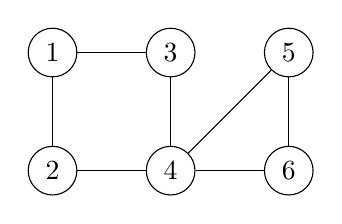
\begin{tikzpicture}[shorten >=1pt,->]
  \tikzstyle{vertex}=[circle, draw]
  \node[vertex] (G_3) at (0,0)   {3};
  \node[vertex] (G_1) at (-1.5,0)  {1};
  \node[vertex] (G_2) at (-1.5,-1.5) {2};
  \node[vertex] (G_4) at (0,-1.5) {4};
  \node[vertex] (G_6) at (1.5,-1.5) {6};
  \node[vertex] (G_5) at (1.5,0) {5};
  
  
  \draw (G_2) -- (G_1) -- cycle;
  \draw (G_1) -- (G_3) -- cycle;
  \draw (G_3) -- (G_4) -- cycle;
  \draw (G_2) -- (G_4) -- cycle;
  \draw (G_5) -- (G_6) -- cycle;
  \draw (G_4) -- (G_5) -- cycle;
  \draw (G_4) -- (G_6) -- cycle;
 
    		\end{tikzpicture}
    		\caption{}
  			\end{subfigure}
  			\hfill
  			\begin{subfigure}[b]{0.45\textwidth}
    		\centering
    		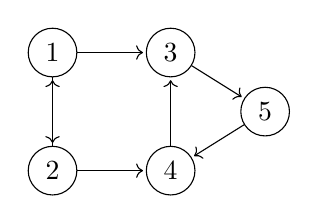
\begin{tikzpicture}[shorten >=1pt,->]
  \tikzstyle{vertex}=[circle, draw]
  \node[vertex] (G_3) at (0,0)   {3};
  \node[vertex] (G_1) at (-1.5,0)  {1};
  \node[vertex] (G_2) at (-1.5,-1.5) {2};
  \node[vertex] (G_4) at (0,-1.5) {4};
  \node[vertex] (G_5) at (1.2,-0.75) {5};
  
  
  \draw (G_2) -- (G_1);
  \draw (G_1) -- (G_2);
  \draw (G_1) -- (G_3);
  \draw (G_4) -- (G_3);
  \draw (G_2) -- (G_4);
  \draw (G_5) -- (G_4);
  \draw (G_3) -- (G_5);
 
    		\end{tikzpicture}
    		\caption{}
  			\end{subfigure}
  \caption{Příklady grafů. (a) Neorientovaný graf. (b) Orientovaný graf.}
  \label{obrazky_grafu}
  \end{figure}
  
			Příklady nakreslení grafu vidíme na obrázku \ref{obrazky_grafu}.
			Pomocí neorientovaného neohodnoceného grafů můžeme například reprezentovat vztahy mezi lidmi, kde vrcholy budou jednotlivé osoby a~hrany povedou mezi těmi dvojicemi vrcholů, které spolu kamarádí. Nebo můžeme pomocí ohodnoceného grafu modelovat síť měst, kde hodnota hran mezi dvěma městy bude značit délku silnice mezi městy. Často se také grafy využívají pro popis \emph{stavového prostoru} her, kde vrcholy představují stavy a~hrany mezi nimi akce, kterými lze přejít z~jednoho stavu do druhého.
			
			
			\subsection{Reprezentace grafu v~počítači}
Existuje několik způsobů, jak efektivně reprezentovat graf v~počítači. %Každá metoda má své výhody a nevýhody, a volba závisí na konkrétních potřebách a vlastnostech grafu. 
Uvedu zde dvě nejběžnější metody použitelné pro jak neorientované, tak orientované grafy. Budou určené pro neohodnocené grafy, ale s~mírnými úpravami se dají použít i~pro ohodnocené grafy.

\begin{itemize}
	\item \emph{Matice sousednosti:} Očíslujeme všechny vrcholy grafu od 1 do $|V|$. Matice sousednosi $A$ má velikost $|V| \times |V|$ a~je definovaná jako $A = (a_{ij})$, kde
	
    $$a_{ij}=
    \begin{cases}
      1 & \text{pokud}\ (i,j)\in E, \\
      0 & \text{jinak}.
    \end{cases}$$
  Výhodou této reprezentace je, že zjistit, zda jsou dva vrcholy spojené hranou zvládneme v~konstantním čase $\mathcal{O}(1)$, vůbec nezáleží na velikosti grafu. Vyjmenování všech následníků vrcholu zabere $\Theta(|V|)$. Nevýhodou je, že zabírá prostor $\Theta(|V|^2)$.
%Pro neorientované grafy je matice symetrická podle hlavní diagonály.
	
	\item \emph{Seznam sousedů:} Vrcholy opět očíslujeme od 1 do $|V|$. Tato reprezentace uchovává pole, které má na $i$-té pozici ukazatel na seznam následníků vrcholu $i$. %$v \in V$ seznam jeho následníků. 
	Tato metoda je efektivnější pro \emph{řídké grafy}, ve kterých $|E| \ll |V|^2$. Zabírá prostor $\Theta(|E|+|V|)$, ale ověřit existenci hrany $(i,j)$ zabere $\mathcal{O}(|V|)$. Výhodou je, že najít všechny následníky vrcholu je lineární s~jejich počtem, tedy $\mathcal{O}(\textrm{počet následníků})$.%$\mathcal{O}(\textrm{počet následníků})$
	

\end{itemize}

%Výběr konkrétní reprezentace závisí na konkrétních požadavcích a prováděných operacích nad grafem. Každá metoda má své vlastní využití a přináší efektivitu při určitých typech algoritmů a operací nad grafy.


			\section{Prohledávání do hloubky}
			Algoritmus prohledávání do hloubky (anglicky \emph{depth-first search}, zkráceně \emph{DFS}) je algoritmus pro procházení grafu. Jak implikuje název, DFS prochází graf vždy tak \emph{hluboko}, jak to jde. DFS začne v~počátečním vrcholu $v_0$ a~prozkoumává vždy následníky naposledy nalezeného vrcholu $v$, z~kterého ještě vedou neprozkoumané hrany. Jakmile narazí na takový vrchol, který nemá žádné neprozkoumané sousedy, nemůže už jít hlouběji a~metodou nazývanou \emph{backtracking} se vrátí na poslední vrchol s~alespoň jedním neprozkoumaným sousedem. Tento proces se opakuje do té doby, než jsou nalezeny všechny vrcholy dosažitelné z~$v_0$.

Pro implementaci algoritmu DFS se využívá datové struktury\footnote{Datová struktura je abstraktní způsob ukládání dat v~počítači umožňující provádět s daty určité operace.} \emph{zásobník}, případně lze použít namísto zásobníku techniku \emph{rekurze}, která stejně využívá systémový zásobník. Zásobník je datová struktura, která si pamatuje pořadí svých prvků, a~řídí se pravidlem LIFO -- Last In, First Out%(doslova "poslední přidaný, první odebraný")
. To znamená, že nové prvky přidává na konec a~odebírá je rovněž z~konce\footnote{Stejně, jako kdybychom chtěli přidat/odebrat náboj ze zásobníku pistole.}. Těmto operacím se obvykle říká PUSH a~POP.

DFS se zásobníkem je popsáno pseudokódem \ref{dfs}.
\begin{algorithm}

			    \caption{Prohledávání do hloubky}
			    \label{dfs}
  				\Vst{Graf $G = (V,E)$, počáteční vrchol $v_0 \in V$}
  				Přidej $v_0$ do zásobníku $Z$ a~označ $v_0$ jako navštívený.
  				
  				\While{zásobník Z~není prázdný}{
				$v \gets$ Z.POP() \Komentar*{Odebere ze zásobníku horní prvek a~uloží ho do $v$}
				\For{ všechny sousedy $w$ vrcholu $v$}{
				\If{$w$ není navštívený}{
				Z.PUSH($w$)
				
				Označ $w$ jako navštívený.
				} 
								
				}
  				}
				%$a\gets x, b\gets y$\;  				
  				%\While{můžeš}{
    			%\If{$a < b$}{prohoď $a$ s $b$}
  				%\If{$b = 0$}{vyskoč z cyklu}
  				%$a \gets a \text{ mod } b$ \Komentar*{mod značí zbytek po vydělení $a$ hodnotou $b$}
  				%}
				
				
				\end{algorithm}
\begin{figure}[h]
\begin{center}
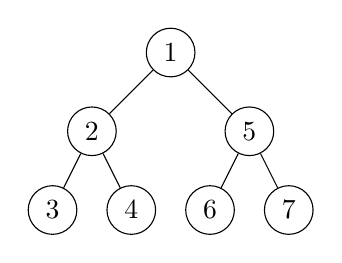
\begin{tikzpicture}[shorten >=1pt,->]
  \tikzstyle{vertex}=[circle, draw]
  \node[vertex] (G_1) at (0,0)   {1};
  \node[vertex] (G_3) at (-1.5,-2)  {3};
  \node[vertex] (G_2) at (-1,-1) {2};
  \node[vertex] (G_4) at (-0.5,-2) {4};
  \node[vertex] (G_5) at (1,-1) {5};
  \node[vertex] (G_6) at (0.5,-2) {6};
  \node[vertex] (G_7) at (1.5,-2) {7};
  \draw (G_1) -- (G_2) -- (G_3) -- cycle;
  \draw (G_1) -- (G_5) -- cycle;
  \draw (G_2) -- (G_4) -- cycle;
  \draw (G_5) -- (G_7) -- cycle;
  \draw (G_5) -- (G_6) -- cycle;
\end{tikzpicture}
\caption{Graf s~vrcholy označenými podle pořadí, v~jakém je projde DFS} \label{grafDFS}
\end{center}
\end{figure}
			Algoritmus \ref{dfs} pouze navštíví každý vrchol dosažitelný z~$v_0$ a~označí ho za navštívený, nic ale nevrací. To proto, že DFS je algoritmus na procházení grafu. Mohli bychom ho ale lehce modifikovat tak, aby našel cestu z~vrcholu $v_0$ do $v_1$. Konkrétně by si pro každý vrchol pamatoval jeho předchůdce a~jakmile by našel cílový vrchol, tak by postupně vypsal cíl, předchůdce cíle atd. Nevýhodou prohledávání do hloubky je, že pokud ho využijeme k~nalezení cesty mezi dvěma vrcholy, nalezená cesta není nutně nejkratší možná, v~důsledku pořadí, v~jakém DFS prochází vrcholy.
			
			 %	DFS lze využít například pro hledání \emph{komponent souvisloti} grafu.
			
			
			Časová komplexita je $\mathcal{O}(|V| + |E|)$, protože v~nejhorším případě projde celý graf. Prostorová složitost je $\Theta(|V| + |E|)$.
			
			\section{Prohledávání do šířky}
			Algoritmus prohledávání do šířky (anglicky \emph{breadth-first search}, zkráceně \emph{BFS}) je dalším algoritmem pro procházení grafu. BFS prochazí graf do \emph{šířky}, tj. postupně prozkoumává všechny sousedy počátečního vrcholu $v_0$, pak sousedy sousedy sousedů  atd. %dříve, než se pohne dál do hloubky.

%Podobně jako u DFS začínáme v počátečním vrcholu $v_0$.
Na rozdíl od DFS používá BFS frontu namísto zásobníku. Fronta je datová struktura, která pracuje podle pravidla FIFO (First In, First Out), což znamená, že prvek, který je ve~frontě nejdéle, bude odebrán jako první. Operaci přidání prvku na konec fronty se obvykle říká ENQUEUE a~odebrání prvku ze začátku fronty DEQUEUE.

Algoritmu se někdy přezdívá \uv{algoritmus vlny}, protože nalezne nejdřív všechny vrcholy vzdálené od $v_0$ o~jedna (sousedy $v_0$), pak ty vzdálené o~dva (sousedy sousedů $v_0$) a~tak dále, jako by se z~$v_0$ šířila vlna po vodní hladině.

Detailní popis nalezneme v~pseudokódu \ref{bfs}.



\begin{algorithm}

			    \caption{Prohledávání do šířky}
			    \label{bfs}
  				\Vst{Graf $G = (V,E)$, počáteční vrchol $v_0 \in V$}
  				Přidej $v_0$ do fronty $Q$ a~označ $v_0$ jako navštívený.
  				
  				\While{fronta Q není prázdná}{
				$v \gets$ Q.DEQUEUE() %\Komentar*{Odebere z fronty první pra uloží ho do $v$}
				
				\For{ všechny sousedy $w$ vrcholu $v$}{
				\If{$w$ není navštívený}{
				Q.ENQUEUE($w$)
				
				Označ $w$ jako navštívený.
				} 
								
				}
  				}
				%$a\gets x, b\gets y$\;  				
  				%\While{můžeš}{
    			%\If{$a < b$}{prohoď $a$ s $b$}
  				%\If{$b = 0$}{vyskoč z cyklu}
  				%$a \gets a \text{ mod } b$ \Komentar*{mod značí zbytek po vydělení $a$ hodnotou $b$}
  				%}
				
				
				\end{algorithm}


\begin{figure}[h]
\begin{center}
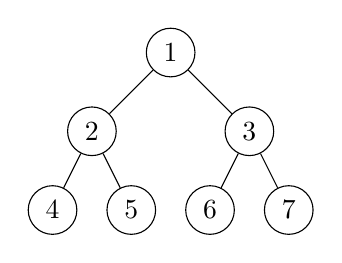
\begin{tikzpicture}[shorten >=1pt,->]
  \tikzstyle{vertex}=[circle, draw]
  \node[vertex] (G_1) at (0,0)   {1};
  \node[vertex] (G_3) at (-1.5,-2)  {4};
  \node[vertex] (G_2) at (-1,-1) {2};
  \node[vertex] (G_4) at (-0.5,-2) {5};
  \node[vertex] (G_5) at (1,-1) {3};
  \node[vertex] (G_6) at (0.5,-2) {6};
  \node[vertex] (G_7) at (1.5,-2) {7};
  \draw (G_1) -- (G_2) -- (G_3) -- cycle;
  \draw (G_1) -- (G_5) -- cycle;
  \draw (G_2) -- (G_4) -- cycle;
  \draw (G_5) -- (G_7) -- cycle;
  \draw (G_5) -- (G_6) -- cycle;
\end{tikzpicture}
\caption{Graf s~vrcholy označenými podle pořadí, v~jakém je projde BFS} \label{grafBFS}
\end{center}
\end{figure}
Časová složitost BFS je $\mathcal{O}(|V| + |E|)$, protože v~nejhorším případě projde celý graf. Prostorová složitost je $\Theta(|V| + |E|)$.

Výhodou BFS je to, že při hledání cesty vždy najde nejkratší\footnote{Takovou, která obsahuje nejméně vrcholů.} cestu mezi dvěma vrcholy, případně pozná, že mezi nimi neexistuje cesta. Protože nijak nezapočítává ohodnocení hran, bude i~v~ohodnocených grafech nacházet cestu s~nejméně vrcholy. V~takových grafech ale jako nejkratší cestu obvykle považujeme tu, která má nejmenší součet ohodnocení všech hran. Z~tohoto důvodu nenalezne BFS optimální cestu na ohodnocených grafech.

%což ho činí vhodným pro hledání nejkratších cest v neohodnocených grafech.
		
			\section{Uspořádané vyhledávání}
			Dosud představené algoritmy jsou primárně určené pro procházení grafů, přestože se dají aplikovat na hledání cesty mezi dvěma vrcholy.
			%, už vůbec nemají žádnou informaci navíc o hledaném vrcholu. 
			Naopak další algoritmy, které představím, jsou zaměřené na hledání optimálních cest, a~to i~v~kladně ohodnocených grafech.
			
			%a jsou \emph{informované}, což znamená, že mají navíc informaci o odhadu vzdálenosti každého vrcholu $v \in V$ od cílového vrcholu. Princip těchto algortimů pochází z intuitivní myšlenky, že pokud budeme hledat nejkratší cestu z Prahy do Brna, nebudeme jako první zvažovat cestu procházející Plzní a podobně.  
			
			%Tento odhad pro každý vrchol typicky zprostředkovává nějaká \emph{heuristická funkce $h(n)$}. 
			
			Tyto algoritmy vybírají, který vrchol \emph{expandovat}\footnote{Expanzí vrcholu myslíme jeho prozkoumání a~přidání jeho neprozkoumaných sousedů do fronty.} jako další v~pořadí podle nějaké evaluační funkce $f : V~\rightarrow \mathbb{R}$. Ta vrací nějakou reálnou hodnotu pro každý vrchol $v \in V$. 
			Hromadně se označují jako algoritmy třídy uspořádaného vyhledávání (anglicky best-first search), protože pořadí, v~jakém prohledávají vrcholy, je nějak uspořádané podle $f$.

			Typicky se jako první prochází vrchol $v$ s~nejmenší hodnotou $f(v)$. K~tomu se často používá prioritní fronta, která řadí své prvky vzestupně podle priority, přiřazené ke každému prvku. Většinou se implementuje pomocí datové struktury \emph{haldy}. Více o~haldách viz \cite{pruvodce}.			
			
			Poznámka: při rešerši na uspořádané vyhledávání jsem se častokrát setkával s~rozlišnou terminologií. V~některých zdrojích \cite{carlos} se jako best first-search označuje algoritmus, který jiní \cite{patel_intro} pojmenovávají jako greedy best-first search. Jiní \cite{uhlik,wiki_best_first,felner} zase považují best-first search jako algoritmický princip nebo třídu algoritmů.
			 %podobně v českých zdrojích se někdy uspořádaným vyhledáváním myslí třída algoritmů, někdy samotné hladové uspořádané vyhledávání. 
			 Já jsem zvolil stejné pojmenování jako \cite{patel_intro, uhlik, felner}, protože mi přišlo nejvíce konzistentní a~logické.
			%určují, v jakém pořadí procházet vrcholy, se označují jako algoritmy třídy uspořádaného vyhledávání. 
			
			
			
			%tzn. rozhodují se, v jakém pořadí prozkoumávat vrcholy na základě nějaké funkce $f(v)$. 

			\subsection{Uniform Cost Search}
			Uniform cost search, dále jen UCS, je algoritmus třídy uspořádaného vyhledávání, který najde optimální %nejlevnější\footnote{Jako nejlevnější cestu označujeme cestu s nejnižším součtem vah všech hran cesty.} 
			cestu mezi počátečním vrcholem $v_0$ a~cílovým vrcholem $c$ v~grafu s~kladně ohodnocenými hranami. 
			UCS funguje podobně jako BFS, jen místo postupného prohledávání vrcholů ve stejné hloubce (se stejným minimálním počtem hran od startu) prohledává UCS ve \uv{vrstvách} stejné ceny.
			
			%UCS funguje velmi podobně jako BFS, jen se místo hladin vrcholů stejně vzdálených od $s$ uvažuje vrcholy se stejným $g(v)$.
			Evaluační funkcí pro UCS je $f(v) = g(v)$, kde $g(v)$ je cena cesty mezi počátečním vrcholem $v_0$ a~vrcholem $v$. 
			UCS používá prioritní frontu, většinou označovanou jako OPEN. Na začátku je do ní vložen pouze počáteční vrchol s~prioritou 0. V~každé iteraci je z~OPEN odebrán vrchol s~největší prioritou a~expandován. Největší prioritu mají prvky s~nejnižší $g(v)$. To znamená, že UCS vždy expanduje vrchol s~nejnižší kumulativní cenou od počátečního vrcholu $v_0$ a~tudíž nalezne optimální cestu do každého vrcholu, protože jinak by už byl vrchol expandovaný po levnější cestě. Expandované vrcholy jsou přidané do seznamu CLOSED. Pro následníky expandovaného vrcholu $v$, kteří nejsou v~CLOSED, je spočítaná jejich $g$ hodnota pro cestu z~vrcholu $v_0$ přes $v$. V~případě, že ještě nejsou v~OPEN, jsou tam přidané s~vypočtenou prioritou. V~opačném případě už v~OPEN jsou s~nějakou $g$ hodnotou, pak pouze pokud je nová $g$ hodnota menší než předešlá $g$ hodnota, je jejich priorita v~OPEN aktualizována.
			
			 V~průběhu běhu algoritmu si budeme pro každý expandovaný vrchol označovat jeho předchůdce. Díky tomu můžeme po nalezení cílového vrcholu rekonstruovat cestu vedoucí z~$v_0$ do $c$.
			
			
			
			%UCS funguje stejně jako Dijkstrův algoritmus, s tím rozdílem že Dijkstrův algoritmus tak, jak je klasicky popisován, zařadí na začátku do prioritní fronty všechny vrcholy s cenou $\infty$, až na $s$, který má cenu $0$.
			Podrobně popsaný je UCS v~pseudokódu \ref{ucs}.
			

			\begin{algorithm}[H]

			    \caption{Uniform cost search}
			    \label{ucs}
  				\Vst{Graf $G = (V,E)$, počáteční vrchol $v_0 \in V$, hledaný vrchol $c \in V$}
  				\Vyst{Seznam $rodice$, uchovávající předchůdce každého nalezeného vrcholu, $g$ uchovávající cenu cesty do každého nalezeného  vrcholu; nebo informaci o~neúspěchu}
  				%Přidej $v_0$ do $OPEN$ \\% a označ $v_0$ jako navštívený.
  				$g(v_0) \gets 0$ \Komentar*{$g(n)$ je cena cesty z~$v_0$ do $n$}
  				Vlož $v_0$ do $OPEN$\\
  				
  				$CLOSE \gets \emptyset$ \Komentar*{$CLOSE$ je prázdný seznam}
  				$rodice(v_0) \gets \emptyset$\\ %\Komentar*{$rodice(v)$ obsahuje předchůdce $v$, skrz kterého vede nejkratší cesta do $v$}
  				%$cena(v_0) \gets 0 $
  				
  				\While{OPEN není prázdný}{
				$u \gets$ OPEN.extractMin() \Komentar*{Odebere z~fronty vrchol s~nejmenší hodnotou $g$ a~uloží ho do $u$}
				
				\If{$u$ je $c$}{
				Vrať $rodice, g$ 
				}
				Vlož $u$ do $CLOSED$\\
				\For{všechny následníky $v$ vrcholu $u$, kteří nejsou v~CLOSED}
				{
				$tmpG \gets g(u) + w(u,v)$ \Komentar*{$w(u,v)$ je váha							hrany $(u,v)$}
				\If{$v$ není v~$OPEN$}{
				$g(v) \gets tmpG$\\
				$rodice(v) \gets u$ \Komentar*{Nastaví vrchol $u$ jako předchůdce $v$}
				Vlož $v$ do $OPEN$
				}
				\ElseIf{$v$ je v~$OPEN$ a~$tmpG$ je menší než $g(v)$}{
				$g(v) \gets tmpG$\\	
				$rodice(v) \gets u$\\
				}
				}

  				}
  				Vrať $nenalezeno$
		\end{algorithm}
				
				Často se setkáme s~podobným algoritmem, nazývaným \emph{Dijkstrův algoritmus}. Ten se od UCS liší minimálně, rozdíly mezi nimi a~argumenty pro používaní UCS v~praxi jsou popsané v~\cite{felner}.
			
			\subsection{Hladové uspořádané vyhledávání}
			Algoritmus hladového uspořádaného vyhledávaní (anglicky \emph{greedy best-first search}) je dalším algoritmem pro hledání cesty v~kladně ohodnoceném grafu. Pracuje na předpokladu, že pokud bude opakovaně \emph{expandovat} vrchol, který je zdánlivě nejblíž k~cílí, najde cestu do cíle nejrychleji. Princip tohoto algoritmu pochází z~intuitivní myšlenky, že pokud budeme hledat nejkratší cestu z~Prahy do Brna, nebudeme jako první zvažovat cestu procházející Plzní a~podobně. 
			%Jinak řečeno předpokládá, že nejkratší cesta povede stejným směrem, jakým je cíl. 
			
			Jedná se o~\emph{informovaný} algoritmus, což znamená, že má navíc informaci o~odhadu vzdálenosti každého vrcholu $v \in V$ od cílového vrcholu. 
			Tento odhad je typicky zprostředkován \emph{heuristickou funkcí $h(v)$}.
			
			%Ideální funkce by pro každý vrchol vrátila jeho skutečnou vzdálenost od hledaného vrcholu, ale takovou funkci obvykle k dispozici nemáme, proto se používají \emph{heuristické funkce}. 
			Heuristické funkce (heuristiky) můžou být jakékoli, pokud např. při hledání cesty mezi dvěma lokacemi budeme znát jejich souřadnice, můžeme je využít pro výpočet heuristiky. %hledáme-li cestu např. mezi městy Evropy nebo na čtverečkovaném papíře s nakreslenými překážkami, často víme o vrcholech grafu, kterým tyto situace reprezetujeme, nejen jejich hrany ale i jejich přesné souřadnice. 

%\subsection{Heuristické funkce}
			Nejčastěji používané heuristické funkce jsou:
			\begin{enumerate}
			
\item \textbf{Eukleidovská vzdálenost:} $h(v) = \sqrt{(x_c - x_v)^2 + (y_c - y_v)^2}$, kde $x_c$,$y_c$ jsou souřadnice cílového vrcholu a~$x_v, y_v$ jsou souřadnice vrcholu $v$. Tuto heuristiku lze použít na grafy reprezentující klasické mapy.

\item \textbf{Manhattanská vzdálenost:} $h(v) = |(x_c - x_v)| +
|(y_c - y_v)|$, kde $x_c$,$y_c$ jsou souřadnice cílového vrcholu a~$x_v, y_v$ jsou souřadnice vrcholu $v$. Tato heuristika je ideální pro mapy reprezentované čtvercovou mřížkou, kde jsou povoleny pouze vertikální a~horizontální pohyby.

\item \textbf{Octile heuristika:} $h(v) = \Delta x+ \Delta y + (\sqrt{2}-2) \cdot min(\Delta x, \Delta y)$, kde $\Delta x = |x_c - x_v|, \Delta y = |y_c - y_v|$. %jsou absolutní rozdíly souřadnic vrcholů, podle souřadnic $x$ a $y$. 
Tato heuristika je ideální pro osmisměrné čtvercové mřížky, tedy takové, kde je kromě vertikálního a~horizontálního pohybu povolen i~diagonální pohyb. Počítá s~cenou 1 pro vertikální a~horizontální pohyby a~cenou $\sqrt{2}$ pro diagonální.
\end{enumerate}
Heuristická funkce $h(n)$ je \emph{přípustná}, pokud pro každý vrchol $v \in V$ platí $h(v) \leq h^*(v)$, kde $h^*(v)$ je \emph{ideální} heuristika, tedy skutečná vzdálenost od cíle.
%Navíc pokud platí i $TODO$, pak funkci označujeme jako \emph{monotónní}.			
			
			
			Pro hladové uspořádané vyhledávání se evaluační funkce rovná heuristické funkci: $f(v) = h(v)$. 						
			
			Na začátku vloží do prioritní fronty počáteční vrchol s~prioritou 0.
			Dokud není prioritní fronta prázdná, tak v~každé iteraci vybere z~prioritní fronty vrchol s~nejmenší $f(v)$ a~ten expanduje, dokud nedorazí do cíle.
			
			Nevýhodou tohoto algoritmu je, že vrcholy prozkoumává jen podle heuristiky. %se snaží jít směrem do cíle, i když tím směrem nemusí vést optimální cesta.
			Jeho efektivita záleží na přesnosti heuristické funkce. Pokud by heuristika byla ideální,  prozkoumá jen vrcholy vedoucí do cíle, a~to po optimální cestě. Jeho evaluační funkce nepřihlíží k~vzdálenosti od počátečního vrcholu a~algoritmus nijak nezohledňuje celkovou ušlou vzdálenost od počátečního vrcholu, což může vést k~nalezení neoptimálních cest. Nicméně nějakou cestu najde většinou rychleji než UCS, protože prozkoumáváním vrcholů zdánlivě bližších k~cíli jako první často sníží celkový počet prozkoumaných vrcholů.
			
			
			%Protože jeho ohodnocovací funkce nijak nezohledňuje vzdálenost od počátečního vrcholu a nijak nepracuje s celkovou ušlou vzdáleností od počátečního vrcholu, vede to k nacházení dlouhých neoptimálních cest.
			
			%má za následek, že algoritmus nenajde vždy optimální řešení
		
			Poznámka: algoritmu se říká hladový, protože jako hladové algoritmy se označují ty algoritmy, které v~každém kroku volí lokální optimum s~vidinou, že tyto volby povedou celkově do globálního optima neboli k~optimálnímu řešení. 			
			%Tímto způsobem se algoritmus velmi agresivně vrhne směrem k cíli, avšak pokud narazí ...dopsat
			
			
			%Toto vede sice rychlému, ale ne vždy optimálnímu hledání. Algoritmus je náchylný k přecenění první cesty, což má za následek nenalezení nejkratší (optimální) cesty.
						
			\subsection{Algoritmus A*}
			Algoritmus A* navrhli Peter Hart, Nils Nilsson a~Bertram Raphael v~roce 1968. % pro jejich robota. 
			Algoritmus A* kombinuje efektivitu hladového uspořádaného vyhledávání s~optimalitou algoritmu UCS.
			
			
			Protože se jedná o~další algoritmus z~třídy uspořádaného vyhledávání, funguje podobně jako UCS i~hladové uspořádané vyhledávání. A* taktéž prochází vrcholy grafu podle hodnoty evaluační funkce a~vybírá vrcholy s~nejnižší hodnotou $f(v)$, jediným rozdílem je evaluační funkce samotná.
			Tento algoritmus jako svou evaluační funkci $f(v)$ využívá součet heuristické funkce $h(v)$ a~funkce $g(v)$, která udává délku nejkratší cesty z~počátečního vrcholu do vrcholu~$v$: $f(v) = g(v) + h(v)$. Heuristika zde figuruje jako informace navíc, kterou čistě z~grafu nevyčteme, proto se i~A* řadí mezi informované algoritmy.  
			
			 
			%Navíc pokud nalezne pro nějaký vrchol kratší cestu z počátku, updatuje jí. 
			
			%Heuristika se přitom volí podle konkrétního problému – např. hledáme-li cestu v mapě, můžeme použít vzdálenost do cíle vzdušnou čarou.
			Pokud bude $h(v)$ přípustná, pak A* vždy najde optimální cestu do cílového vrcholu.		
			 Zvolit přípustnou heuristiku bývá jednoduché, stačí aby nikdy nepřecenila skutečnou cenu cesty do cíle. Například pro hledání cesty v~mapě můžeme použít vzdálenost do cíle vzdušnou čarou neboli eukleidovskou vzdálenost. Ovšem čím menší $h(v)$ bude tím více vrcholů A* prozkoumá. 
			
			Pokud bychom zvolili takovou heuristiku, že $\forall v~\in V:h(v) = 0$ tak A* degraduje do UCS, naopak pokud $\forall v~\in V:g(v) = 0 $ tak A* degraduje do hladového uspořádaného vyhledávání řízeného pouze heuristikou.
			
			
			
			A* je velmi populární volbou pro implementaci pathfindingu ve hrách nebo v~mapových aplikacích pro jeho optimalitu a~zároveň efektivitu a~rychlost výpočtu. Existují i~optimalizované verze A*, které například omezují paměťové nároky.
			
			
			
	
	\part{Implementace vizualizačního programu}
		
		\chapter{Záměr práce}
			Cílem druhé části této práce je vytvoření vizualizačního programu, který bude sloužit k~názornému ilustrování chodu algoritmů popsaných v~předchozí části. Při tvorbě programu bude kladen důraz na lehce osvojitelné ovládání, které umožní komukoliv používat program bez nutnosti školení.
			
			Vizualizační program bude navržen tak, aby uživatelům umožnil pohodlně a~jednoduše upravovat veškeré vstupní parametry vizualizace. Taková míra interaktivity dovolí uživateli zkoumat chování algoritmů na různých grafech a~objevovat jejich silné a~slabé stránky.
			 Primárním záměrem programu je pak pomoci studentům nebo případným zájemcům o~problematiku vyhledávání cest do hloubky porozumět principům za jednotlivými algoritmy pro hledání cest.
			 %Tato část se zabývá představením použitých technologií, popisem aplikace a jejích funkcí a příručky jak ji používat.
			 
			 %Mým cílem je i dovolit hodně velké grafy protože je to cool.

		\chapter{Plánování}
			Vizualizace je proces vytváření obrazu něčeho, co není zrovna vidět nebo nějakého abstraktního konceptu. Algoritmy jsou abstraktními koncepty z~definice. Co víc, i~když si algoritmus úspěšně naprogramujeme, typicky nevidíme a~ani nesledujeme každý jeho krok, zajímá nás jen výsledek. To je pochopitelné, pokud algoritmu rozumíme a~používáme ho k~řešení konkrétního problému. Naopak hlavním smyslem vizualizace algoritmu je názorně ilustrovat chod algoritmu, zejména pro výukové účely.
			%Vizualizace tedy slouˇz´ı k lepˇs´ımu pochopen´ı probl´emu, kter´y modeluje
			\section{Reprezentace grafu}
			Než se pustíme do samotného programování vizualizační aplikace, musíme si nejprve promyslet, jak si vůbec vizualizační program představujeme. 
			Jelikož je účelem programu vizualizovat grafové algoritmy, je jedním z~nejdůležitějších rozhodnutí, jakým způsobem graficky reprezentovat graf. Nabízí se možnost grafy reprezentovat podobně jako na obrázku \ref{obrazky_grafu}. Avšak takový přístup by značně omezil a~ztížil uživateli návrh vlastních grafů, protože by musel každý jeden vrchol manuálně vytvořit a~zdlouhavě propojovat vybrané vrcholy hranami. Pro větší počet vrcholů už by se vizualizace mohla značně znepřehlednit. Od vizualizace požadujeme i~možnost zobrazovat \uv{velké} grafy, protože na grafu s~malým počtem vrcholů by vizualizace nemusely být dostatečně názorné.
			
			Proto budeme reprezentovat graf pomocí mřížky. Na mřížku lze nahlížet jako na speciální druh grafu, kde každé políčko mřížky bude reprezentovat vrchol a~mezi sousedními políčky povedou pomyslné hrany. Takový graf sám o~sobě by byl velmi jednotvárný a~nezajímavý, proto do mřížky půjde umísťovat neprůchodné stěny, které graf zredukují o~některé prvky. 
			
			Jednou možností, jak realizovat stěny, je nechat všechna políčka průchozí a~umisťovat stěny mezi některé sousední políčka, což bude v~grafu ekvivalentní se smazáním hran mezi odpovídajícími vrcholy. Druhou možností je určit některá políčka jako stěny a~odpovídající vrcholy z~grafu smazat, stejně jako všechny hrany, jichž jsou součástí. 
			
			Pro náš program zvolíme druhou možnost, protože takovou mřížku půjde jednoduše upravovat. Ukázka takové mřížky je na obrázku \ref{mrizka_ukazka}. Uživatel si bude moct vybrat nástroj štětce a~tím označit políčka, která mají figurovat jako stěny. Další nutné nástroje zahrnují nástroje pro umisťování a~přemísťování startovních a~cílových vrcholů. 
			
			\begin{figure}
  			\centering
  			\begin{subfigure}[b]{0.45\textwidth}
  			\centering 
  			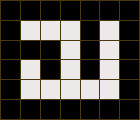
\includegraphics{mrizka2.png}
  			\caption{}
  			\end{subfigure}
  			\hfill
  			\begin{subfigure}[b]{0.45\textwidth}
    		\centering
    		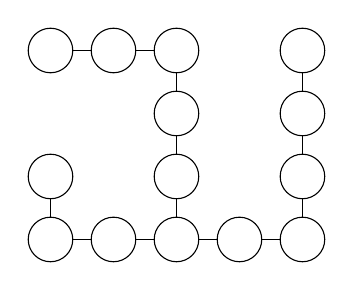
\begin{tikzpicture}[node distance={8mm},shorten >=1,->]
  \tikzstyle{vertex}=[circle, draw, inner sep=2mm]
  \node[vertex] (1) at (0,2) {};
  \node[vertex] (2) [left of=1]  {};
  \node[vertex] (3) [left of=2]  {};
  \node[vertex] (4) [left of=3]  {};
  \node[vertex] (5) [left of=4]  {};
  \node[vertex] (6) [above of=5]  {};
  \node[vertex] (7) [above of=3]  {};
  \node[vertex] (8) [above of=1]  {};
  
  \node[vertex] (9) [above of=7]  {};
  \node[vertex] (10) [above of=8]  {};
  
  \node[vertex] (11) [above of=9]  {};
  \node[vertex] (12) [above of=10]  {};
  
  \node[vertex] (13) [left of=11]  {};
  \node[vertex] (14) [left of=13]  {};
  
  \draw (1) -- (2) -- (3) -- (4) -- (5) -- cycle;
  \draw (1) -- (8) -- (10) -- (12) -- cycle;
  \draw (3) -- (7) -- (9) -- (11) -- (13) -- (14) -- cycle;
  \draw (5) -- (6) -- cycle;
 
    		\end{tikzpicture}
    		\caption{}
  			\end{subfigure}
  \caption{(a) Mřížka v~aplikaci, černá políčka jsou stěny. (b) Odpovídající graf.}
  \label{mrizka_ukazka}
  \end{figure}			

		
		\section{Výběr algoritmů}
						
			Poslední důležitou volbou bylo, které všechny algoritmy bude program schopen vizualizovat. Těmito vybranými algoritmy se staly DFS, BFS, hladové uspořádané vyhledávání a~A*. Algoritmus UCS vynecháme z důvodu, že na neohodnocených grafech prohledává velmi podobně jako BFS. Mřížka v programu odpovídá neohodnocenému grafu, protože jako sousedy vrcholu bude považovat jen ty políčka sousedící ve vertikálním a~horizontálním směru. Cena přechodu z~jednoho políčka do druhého tak bude vždy stejná. Jako heuristika bude použita manhattanská vzdálenost, protože je pro takovéto mřížky nejvhodnější.
			
			%protože manuální tvoření vlastního grafu po jednom vrcholu zní náročně.
			%Cílem je předání dané informace co nejsrozumitelnější formou.
			\section{Výběr prostředků pro vizualizaci}
			Dalším krokem bylo zvolit si vhodné softwarové nástroje pro implementaci takového programu. Já se rozhodl pro programovací jazyk Python, protože umožňuje poměrně rychlý vývoj a~mám s~ním největší zkušenosti.
			
			%však pro mé potřeby však nenabízí dostatečně dobré , proto 
			Samotný Python musíme doplnit nějakou knihovnou pro práci s~GUI\footnote{Z anglického \emph{Graphical User Interface}.} -- grafickým uživatelským rozhraním. Pro tento účel zvolíme knihovnou \texttt{pygame}. \texttt{Pygame} je populární knihovna primárně určena pro vývoj her.  
			%Umožňuje snadné vykreslování na obrazovku, zachycování vstupu a podobně. 
			Pygame je postavena nad knihovnou Simple DirectMedia Layer (SDL), která obsluhuje nízkoúrovňové úlohy jako je renderování grafiky, zpracování zvuku a~zachycování vstupu. Díky tomu se při vývoji s~pygame můžeme zaměřit na implementaci logiky celé aplikace a~nemusíme řešit tyto nízkoúrovňové záležitosti.
			%očekával jsem že i moje aplikace s její pomocí půjde implementovat. 
			Nesmírnou výhodou pygame je její jednoduchost v~kombinaci s~množstvím dostupných online tutoriálů, vysvětlujících jak základní principy, tak pokročilou práci s~knihovnou.
			\cite{pygame_intro} \cite{pygame_about}
			 %neposlední řadě je skvělá pygame dokumentace \cite{pygame_dokumentace}. \cite{pygame_about} 			
			
		
		\chapter{Vlastní vývoj}
		V~této kapitole si představíme hotový program a~jednotlivé soubory, z~kterých se skládá. Celý zdrojový kód je uveden v~příloze, rovněž je dostupný na adrese \url{https://github.com/alexandrBihun/Maze-Visualizer/releases/tag/MaturitniPrace}.
			\section{Struktura programu}
			Pro základní strukturu pygame programu mi byl inspirací \cite{yt_zelda}. Program je rozdělen podobným způsobem na jednotlivé moduly, které spolu komunikují. Každý modul obsahuje třídy a~funkce zaměřené na jeden aspekt programu podle objektově orientovaného paradigmatu. Diagram modulů, tříd a~jejich vzájemných interakcí vidíme na obrázku \ref{app_diagram}. Každý modul vyjma \texttt{sidebar.py} obsahuje jednu třídu. Modul \texttt{settings.py} představuje pouze konfigurační soubor s~nastavením pro celý program.
			
			\subsection{Modul \texttt{main.py}}
			Soubor \texttt{main.py} slouží jako vstupní bod celé aplikace, pomocí kterého se aplikace spouští. Definuje třídu \texttt{AppMain}, která reprezentuje celou aplikaci. Tato třída inicializuje knihovnu pygame a~vytváří si instanci třídy \texttt{Vizualizator}. \texttt{AppMain} definuje hlavní programovou smyčku a~je zodpovědná za ošetřování veškerých uživatelských událostí. Většinu událostí pak předává ke zpracování instanci \texttt{Vizualizator}. 

			\subsection{Modul \texttt{vizualizator.py}} \label{subsection}
			Tento modul tvoří jádro celé aplikace, zatímco všechny ostatní mají pouze podpůrnou roli vůči tomuto modulu.
			Definuje třídu \texttt{Vizualizator} s~množstvím atributů a~řadou metod. 
			
			Třída uchovává celý graf ve 2D~seznamu čili seznamu seznamů v~proměnné \texttt{grid}. Prvky v~něm lze indexovat jako \texttt{grid[x][y]}, každý prvek v~\texttt{grid} je instancí třídy \texttt{Tile} z~modulu \texttt{tile.py}. Dále uchovává instanci třídy \texttt{Sidebar} a~několik atributů určujících stav programu jako je vybraný nástroj, vybraný algoritmus, rychlost vizualizace, pozice startu a~cíle několik dalších méně důležitých atributů. Za zmínku stojí atribut \texttt{coloredSearch}. %který určuje zda bude vizualizace běžná nebo bude využívat barevný přechod. 
			Pokud je nastavený na \texttt{True}, budou se při vizualizaci každého algoritmu používat pro nalezená políčka různé barvy, konkrétně takové, že každý nalezený vrchol bude mít nepatrně pozměněný odstín barvy oproti svému předchůdci. Tím vznikne efekt barevného přechodu a~možnost pro hlubší analýzu algoritmů.
			
			Základní metody třídy \texttt{Vizualizator}:
			\begin{itemize}
			\setlength\itemsep{0.01mm}
			\item \texttt{initGrid()}\\
			Inicializuje \texttt{grid} a~naplní ho \texttt{Tile} objekty, stanový prvotní startovní a~cílový vrchol.
\item \texttt{run()}\\
Volá se každý snímek a~překreslí obrazovku, pokud uživatel v~posledním snímku editoval stěny.
\item \texttt{handleEvents(event)}\\
Obsluhuje veškeré události, zejména stisky klávesnice a~kliknutí myši. V~případě stisklého tlačítka myši volá metody z~\texttt{Tools.py} pro upravení stěn.

\item \texttt{space\_pressed()}\\
Obsluha události stisknutí mezerníku, provede celou vizualizaci. Konkrétně volá \\ \texttt{redrawVisited}, \texttt{runVisualiztion} a~\texttt{visualizePath}.

\item \texttt{redrawVisited(redrawAll)}\\
Překreslí všechna políčka vybarvená předešlou dokončenou vizualizací na původní barvu. Pokud je \texttt{drawAll} \texttt{True}, překreslí všechna políčka s~jejich aktuální barvou. Druhé možnosti se využívá při přepnutí vykreslování čar mřížky.
\item \texttt{runVisualization()}\\
Spustí vizualizaci dle vybraného algoritmu.

\item \texttt{visualizePath(path: dict, found)}\\
Rekurzivně vizualizuje nalezenou cestu z~cílového vrcholu. Zároveň spočítá její délku a~počet polí navštívených během vizualizace a~tyto údaje předá metodám z~třídy \texttt{Sidebar}.


\item \texttt{changeVisualizationSpeed(event)}\\
Obsluha události stisknutí šipky nahoru nebo dolů, změní rychlost vizualizace. Buďto upravuje časovou prodlevu mezi kroky algoritmu nebo při dosažení prodlevy nula, kdy se kreslí jeden krok za snímek, zvětšuje počet kroků vizualizovaných v~jednom snímku.

\end{itemize}
Metody pro všechny algoritmy:
\begin{itemize}
			\setlength\itemsep{0.01mm}
\item \texttt{DFS()}
\item \texttt{BFS()}
\item \texttt{greedy\_BeFS()}
\item \texttt{aStar()}\\
Pro vizualizaci algoritmů byl zvolen \uv{polointeraktivní} způsob vizualizace. Algoritmy se vizualizují za běhu a~mezi každými dvěma kroky čekají nějakou stanovenou dobu. Kvůli tomu není možné algoritmus manuálně krokovat. Na druhou stranu program umožňuje před i~během vizualizace měnit tuto časovou prodlevu, takže si uživatel může nastavit delší prodlevu a~důkladněji pozorovat jednotlivé kroky algoritmu. Zdrojový kód pro všechny implementované algoritmy se nachází v příloze \ref{idk}. 
\end{itemize}

Pomocné metody pro algoritmy:
\begin{itemize}
\setlength\itemsep{0.01mm}
\item \texttt{manhattan\_dist(node, goal)}\\
Spočítá hodnotu manhattanské vzdálenosti z~\texttt{node} do \texttt{goal}.
\item \texttt{setCurrsColour(current, parentDict)}\\
Nastaví právě prozkoumanému vrcholu novou barvu.
\item \texttt{algo\_visualize(i)}\\
Vizualizuje další krok algoritmu podle nastavené rychlosti vizualizace.






\item \texttt{Alg\_check\_events()}\\
Ošetřuje události během  běžící vizualizace. Každý algoritmus ji volá jednou za krok. 
\item \texttt{color\_shift(rgb)}\\
Mírně posune odstín barvy na vstupu, přičemž jí ponechá původní saturaci a~jas. Využíváno při barevné vizualizaci algoritmů.
\end{itemize}

Zbylé metody:
\begin{itemize}
			\setlength\itemsep{0.01mm}
\item \texttt{drawGrid()}\\
Nakreslí všechny čáry určující mřížku. Pozice čar jsou spočítané v~atributu \\ \texttt{gridLinesDistribution}. Výhodou tohoto přístupu oproti kreslení všech políček s~okraji je, že pokud počet políček nedělí délku mřížkové oblasti v~pixelech, budou čáry rovnoměrně rozložené po celé oblasti. Při kliknutí uživatele pouze určíme, mezi které čáry klikl. Dále nemusíme složitě rozhodovat které políčka by se měla nakreslit o~něco užší než ostatní, tak aby se všechna políčka vešla do mřížkového prostu a~měla zdánlivě stejnou velikost.
\item \texttt{generateMaze()}\\
Vygeneruje náhodné bludiště pomocí Primova randomizováného algoritmu. Při implementaci jsem postupoval podle \cite{prim}.
Algoritmus funguje tak, že označí všechna políčka až na jedno náhodné za stěny. Tomuto vybranému poli určí \emph{frontiery}, vrcholy, které jsou stěna a~nachází se ve vzdálenosti dva od vybraného políčka. Udržuje si seznam všech nalezených frontierů a~dokud není prázdný opakuje jeden krok: odeber náhodného frontiera ze seznamu a~nastav ho a~políčko mezi ním a~rodičovským vrcholem jako průchozí a~přidej frontiery právě vybraného frontiera do seznamu frontierů. Graf reprezentující takto vygenerované bludiště má vlastnost \emph{stromu}: mezi každou dvojicí vrcholů vede právě jedna cesta \cite{pruvodce}. Takováto bludiště se označují jako \emph{perfektní} \cite{maze}.
		
\end{itemize}
			
			
			\subsection{Modul \texttt{tile.py}}
			V~tomto modulu se nachází třída \texttt{Tile} reprezentující jednotlivá políčka v~mřížce. Instance \texttt{Tile} má atributy souřadnic \texttt{x} a~\texttt{y}, pravdivostní hodnotu určující status stěny, cíle nebo startu a~atribut \texttt{colour} určující, jak se má vykreslit na obrazovku. Definuje metodu \texttt{get\_neighbours}, vracející své sousedy v~pořadí jih, sever, západ, východ a~pokud je součet \texttt{x} a~\texttt{y} tohoto vrcholu dělitelný dvěma, pořadí sousedů je otočeno. Tím je při vizualizaci docíleno nalézání \uv{hezčích} cest, které preferují střídání vertikálních a~horizontálních kroků oproti dlouhým sekvencím pouze horizontálních a~pouze vertikálních kroků. Toto řešení představuje \cite{patel_implementation}. Dále metodu \texttt{drawSelf} pro nakreslí sama sebe na obrazovku.
			
			
			
			\subsection{Modul \texttt{tools.py}}
			Modul \texttt{tools.py} je zodpovědný za fungování nástrojů používaných k~umisťování a~mazání stěn, rovněž jako k~přesouvání startovních a~cílových vrcholů. Definuje třídu \texttt{Tools} se statickými metodami\footnote{Statická metoda je přiřazena k~celé třídě jako takové, ne konkrétním instancím.}:
			\begin{itemize}
			\setlength\itemsep{0.01mm}
			\item \texttt{\_getCellPos(mousePos)}\\
			Převede pozici kurzoru myši na souřadnice políčka, na kterém leží kurzor.
			\item \texttt{setWall(mousePos, grid, drawnTiles)}\\
			Změní status \texttt{isWall} poli určenému pozicí kurzoru po kliknutí.
			\item \texttt{setWallCurve(mousePos, grid, drawnTiles, rel)}\\
			Jako minulá metoda jen řeší kreslení a~mazání stěn při pohybu myši se stisklým tlačítkem.
			\item \texttt{switchWall(tile)}\\
			Pomocná metoda využívaná předchozími dvěma metodami.
			\item \texttt{setEndPoints(mousePos, grid, currEndPointPos, start=False, goal=False)}\\
			Určí nový vrchol jako konečný, podle parametru buď startovní nebo cílový.
			\end{itemize}						

			
			Zajímavým problémem bylo, jak vyřešit kreslení stěn při rychlých pohybech kurzoru. Důvodem je, že události od uživatele můžeme zpracovat jen jednou za každý snímek programu, takže pokud se kurzor přesouvá velmi rychle, často se stane že na jednom snímku je umístěný na jednom políčku a~na dalším snímku je už umístěný na úplně jiném, nesousedním políčku. Z~pohledu uživatele to vypadá tak, že se myš přesouvala plynule po jednotlivých polích a~proto očekává že se překreslí všechna. Kdybychom ale kontrolovali pozici stisklé myši jen jednou každý snímek, nezaznamenali bychom všechna pole, přes která bylo kresleno. Naštěstí \texttt{pygame} událost pro pohyb kurzoru udává i~relativní změnu od minulé pozice kurzoru. Díky tomu můžeme k~první pozici plynule připočítávat malé díly této relativní změny a~zaznamenat všechna překreslená pole. Další důležitou poznámkou je, že metoda je ošetřená tak, aby buďto pouze mazala nebo kreslila stěny, což má za následek předvídatelné chování. Je nežádoucí, aby se při jednom souvislém pohybu myši se stisklým tlačítkem zároveň mazaly i~umisťovaly stěny.
			
			\subsection{Modul \texttt{sidebar.py}}
			Tento modul definuje třídu \texttt{Sidebar} reprezentující boční panel aplikace. Dále pak pomocné třídy \texttt{Text} a~\texttt{Button} pro zobrazovaní textu a~tvorbu tlačítek, protože \texttt{pygame} samotná neobsahuje žádné podobné třídy. Třída ukládá instance \texttt{Button} a~\texttt{Text} pro každý zobrazovaný element a~je jednoduché pomocí pomocných tříd přidávat další.
			Metody třídy \texttt{Sidebar}:
			
			\begin{itemize}
			\setlength\itemsep{0.01mm}
			\item \texttt{redraw\_sidebar(self)}\\
			překreslí celý boční panel
			\item \texttt{print\_path\_len(self, path\_len)}\\
			vypíše do odpovídajícího textového pole délku cesty nalezené dokončenou vizualizací
			\item \texttt{print\_num\_visited\_tiles(self, num\_visited)}\\
			vypíše do odpovídajícího textového počet prozkoumaných polí
			\item \texttt{handle\_events(self, event)}\\
			obsluhuje události kliknutí na tlačítko
			\item \texttt{set\_selected\_algo(self, selectedAlgo)}\\
			změní vybraný algoritmus a~přepíše tuto informaci v~odpovídajícím textovém poli
			\end{itemize}
			
			
			%Třída \texttt{Sidebar} je zodpovědná za vykreslování délky cesty nalezené dokončenou vizualizací pomocí metody \texttt{print\_path\_len(self, path\_len)} a počtu prozkoumaných polí pomocí \texttt{print\_num\_visited\_tiles(self, num\_visited)}. Dále se stará o obsluhu kliknutích na tlačítka metodou \texttt{handle\_events(self, event)}. Posledními metodami jsou\\ \texttt{redraw\_sidebar(self)}, která překreslí celý boční panel a \\ \texttt{set\_selected\_algo(self, selectedAlgo)}, která změní vybraný algoritmus a přepíše tuto informaci v odpovídajícím textovém poli.
			
			\subsection{Modul \texttt{settings.py}}
			Modul \texttt{settings.py} figuruje jen jako konfigurační soubor, umožňující změnit hlavní nastavení celého programu. Nejdůležitějším nastavením je \texttt{sideLength} určující počet polí v~mřížce, dále lze nastavit rozlišení a~barvy polí.
			
			\begin{figure}[H]
  			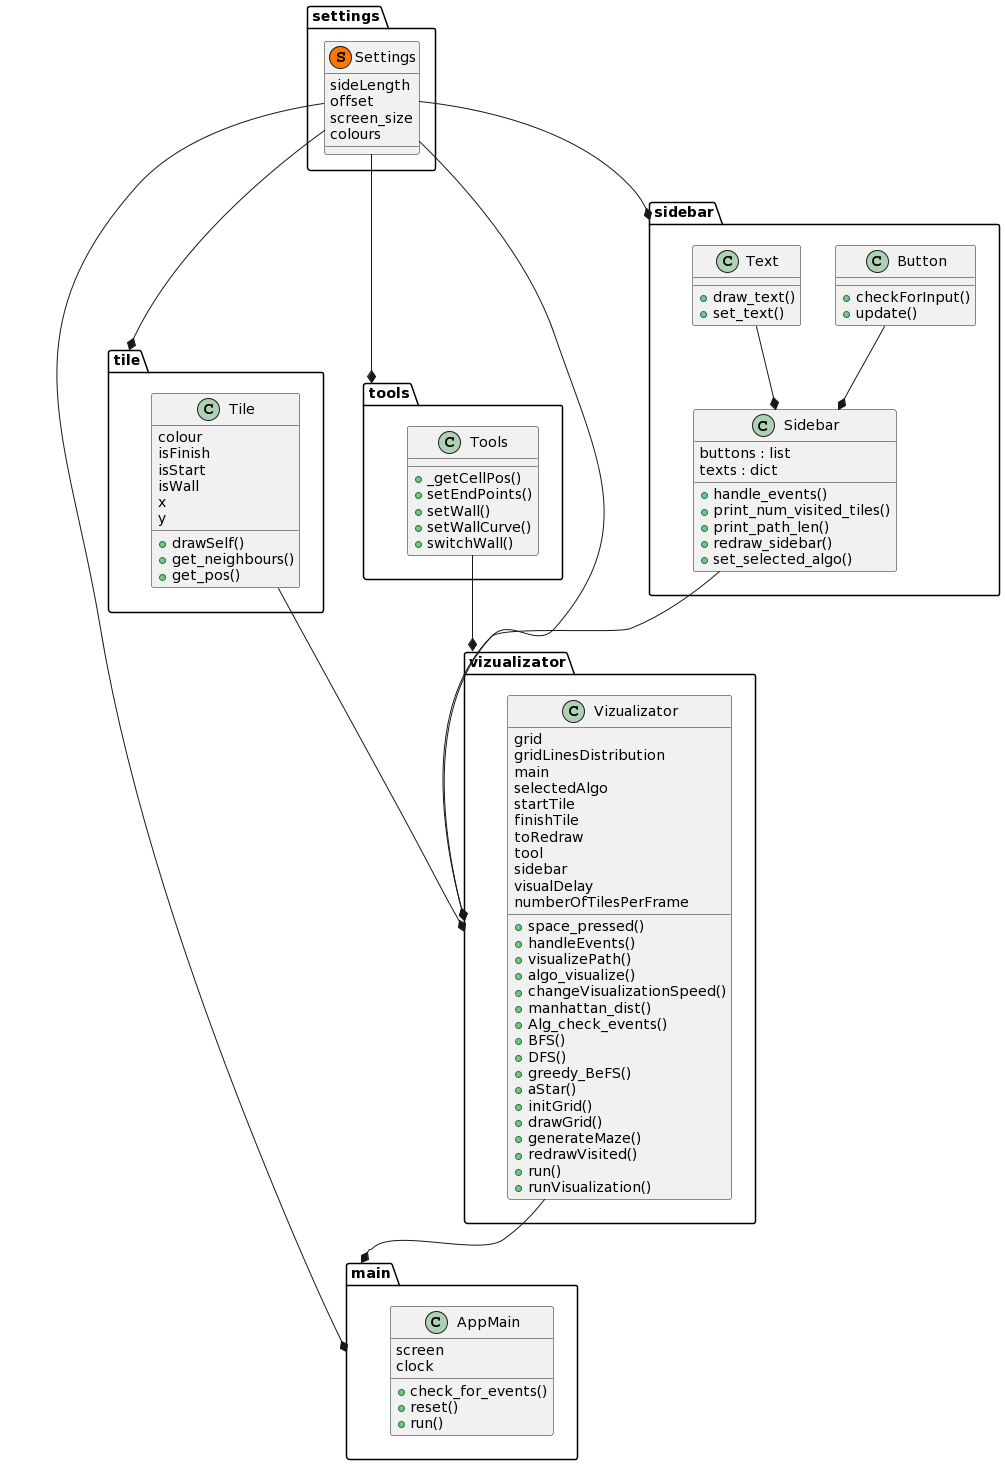
\includegraphics[height=\textwidth,angle=90,origin=c]{diagram2}\caption{Diagram modulů a~tříd}\label{app_diagram}\end{figure}
  			\newpage
  			
		\section{Poznámky k~implementaci}
		Díky mému zvolenému postupu je možné libovolně škálovat počet polí v~mřížce, předvídatelně se program chová až do velikosti jednoho pixelu na políčko. Trochu nečekaně se program na velkých grafech stal jistou imitací grafických editorů jako je MS Paint. Ukázku kreslení na takto velké mřížce ukazuje obrázek \ref{hello}.
		\begin{figure}[h]
		  			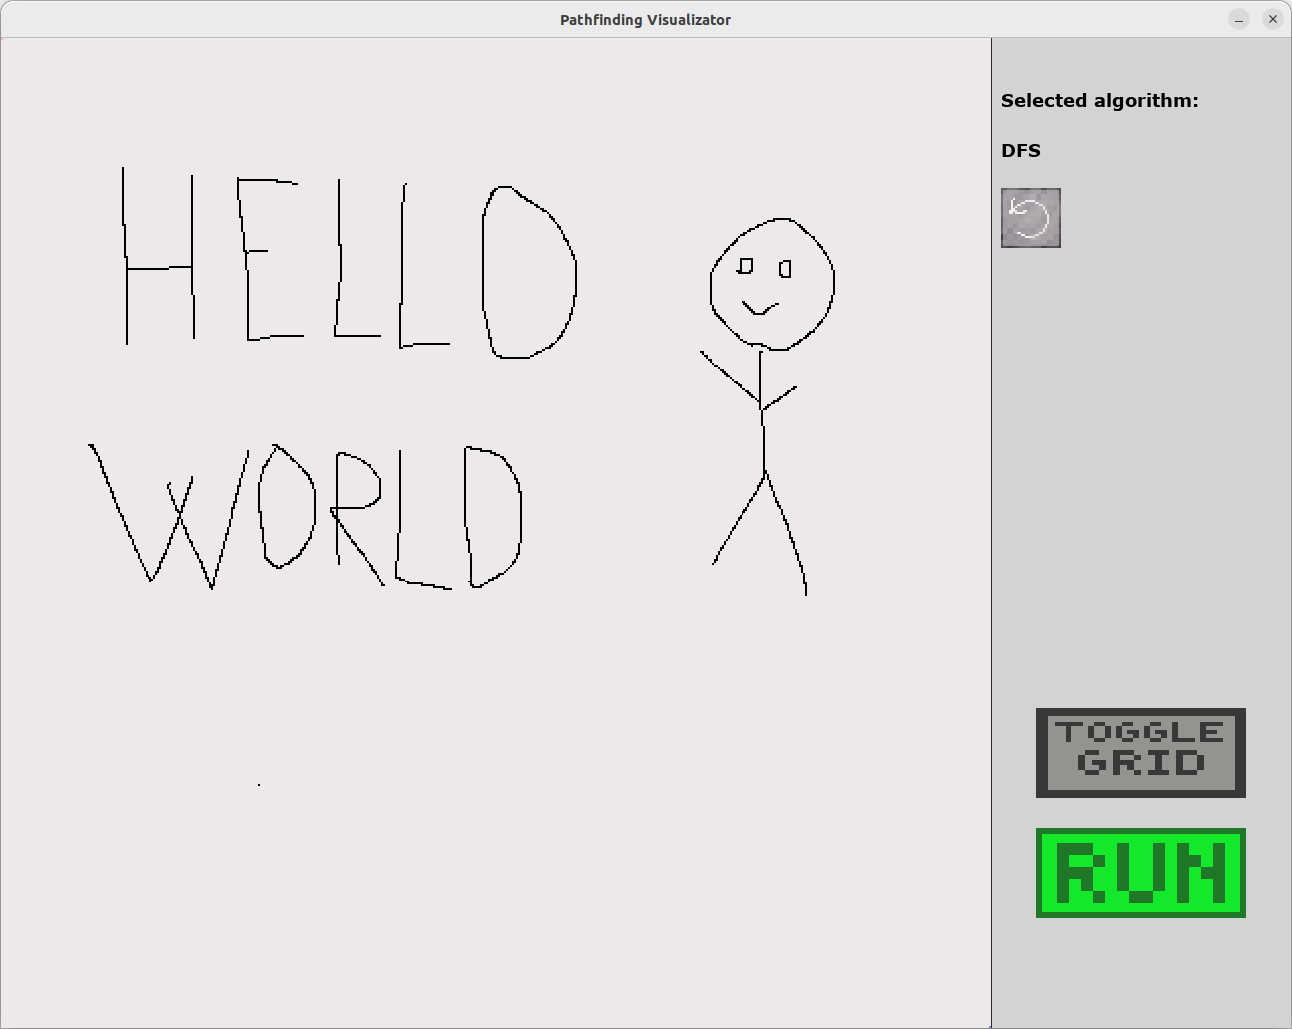
\includegraphics[width=0.99\textwidth]{hello_world}\caption{Aplikace s~nastavením \texttt{sideLength} = 500 a~nakresleným textem.}\label{hello}\end{figure}
		
		Dalším bodem, který musím okomentovat, je možnost barevné vizualizace algoritmů. Protože jako způsob provedení tohoto barevného přechodu bylo zvoleno postupné měnění odstínu podle modelu HSV\footnote{Barevný model se složkami Hue, Saturation, Value.}, výsledné barvy se opakují a~není možné říct, že všechna políčka se stejným odstínem mají nějakou společnou vlastnost jako např. stejnou vzdálenost od počátečního vrcholu. Přesto však poskytuje tato vizualizace informaci navíc o~způsobu, jakým algoritmus prohledává a~speciálně při použití barevného BFS hodnotnou informaci o~struktuře nakresleného nebo vygenerovaného bludiště. 
		
		Na obrázku \ref{bludiste_barvy} je zobrazena vizualizace barevného BFS na bludišti vygenerovaném Primovým randomizovaným algoritmem. Je zřejmé, že i~přesto, že se bludiště jeví jako náhodné, lze v~něm pozorovat vysokou úroveň uspořádanosti. Konkrétně obsahuje soustředné kruhy se stejnou vzdáleností od středu. Tímto středem je vždy první náhodně vybraný vrchol. %Protože skrz %Z vizualizace je patrné, že právě kořen stromu se nachází vždy v prvním vybraném vrcholu.
		
\begin{figure}[h]
\begin{minipage}[outer sep=0]{\textwidth}
\begin{minipage}[t]{0.48\textwidth}
			
  			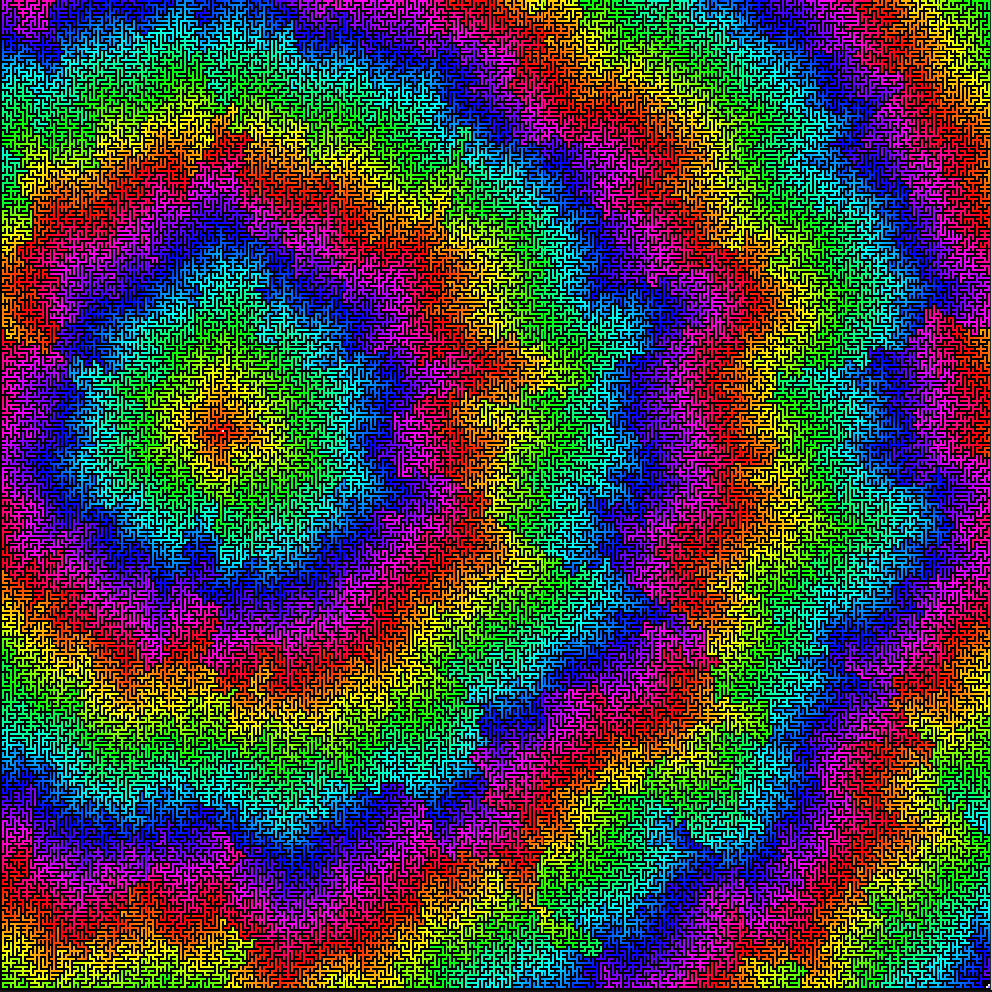
\includegraphics[width=\textwidth]{bludiste_barvy}\caption{Bludiště Primova randomizovaného algoritmu obarvené algoritmem BFS, spuštěným z~prvního vrcholu vybraného pro zbourání stěny.}\label{bludiste_barvy}
  			
    \end{minipage}\hfill
    \begin{minipage}[t]{0.48\textwidth}
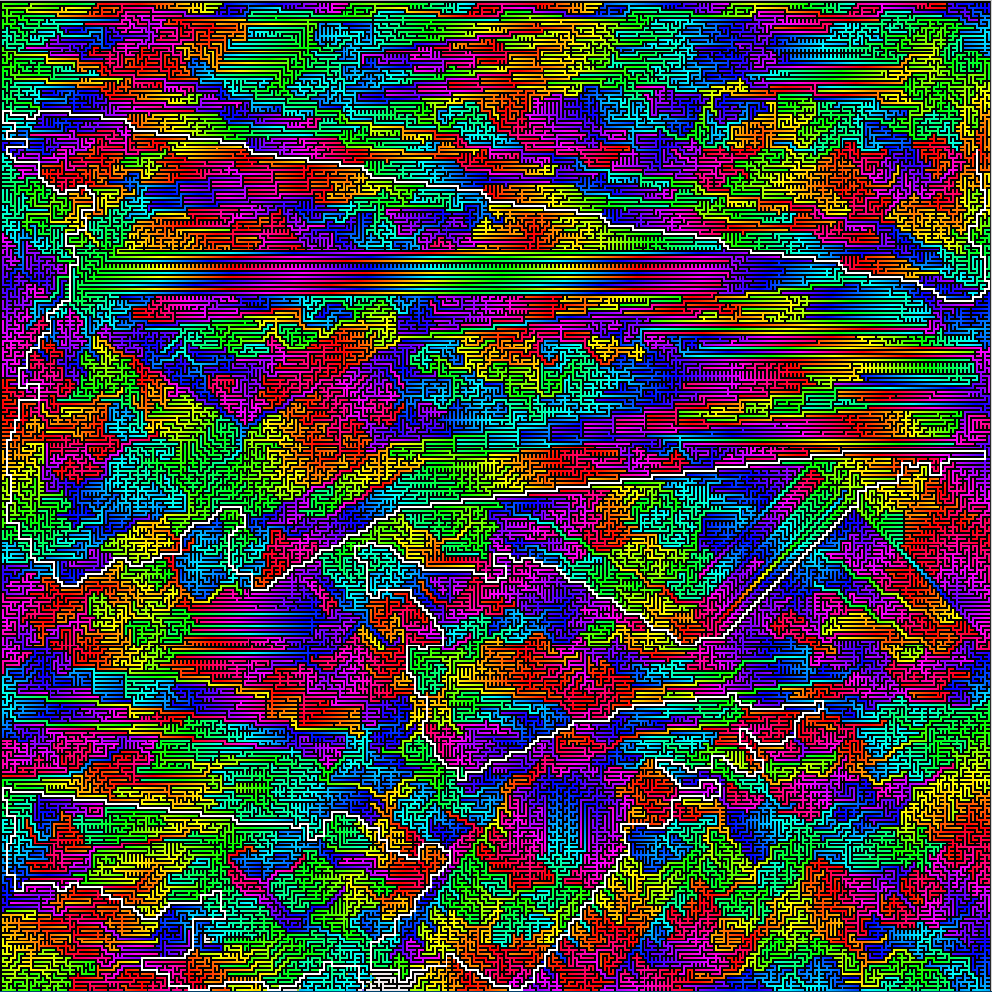
\includegraphics[width=\textwidth]{bludiste_barvy_edit}\caption{Bludiště upraveného Primova randomizovaného algoritmu obarvené algoritmem BFS, spuštěným z~prvního vrcholu vybraného pro zbourání stěny.}\label{bludiste_barvy_edit}
    \end{minipage}
    \end{minipage}\vspace{1ex}
\end{figure}
  			
		%Algoritmus funguje tak, že označí všechny políčka až na jedno ze stěny. Pak z si udržuje seznam všech 
		
		Při náhodných pokusech jsem narazil na způsob, jak upravit algoritmus na generování bludiště tak, aby vygenerované bludiště obsahovalo delší a~klikatější cesty. Konkrétně místo odebírání náhodného vrcholu ze seznamu frontierů\footnote{Viz metoda \texttt{generateMaze() v sekci \ref{subsection}}.} odebere frontiera podle kódu:
		\lstset{numbers=none}
 		\begin{lstlisting}[language = Python]
            var = 10
            if len(frontiers) >= var:
                randomTile = frontiers.pop(-var)
            else: randomTile = frontiers.pop()
		\end{lstlisting}
		oproti původnímu:
				\begin{lstlisting}[language = Python]
randomTile = frontiers.pop(random.randint(0, len(frontiers) - 1))
		\end{lstlisting}
		\lstset{numbers=left}
		Namísto náhodného výběru políčka se tak vybírá většinou políčko které je desáté poslední přidané do seznamu. Navíc je třeba přidat při vkládání frontierů do seznamu kontrolu duplikátů, jinak algoritmus nedoběhne.
		Tato upravená verze algoritmu rovněž vytvoří graf, který je stromem.
		
		Na obrázku \ref{bludiste_barvy_edit} je zobrazené takto vygenerované bludiště prohledané algoritmem BFS spuštěným z~prvního vrcholu vybraným generovacím algoritmem. Toto bludiště vykazuje větší míru náhodných dlouhých cest a~méně uspořádanosti. Díky tomu na takto vygenerovaném bludišti budou mít A* a~hladové uspořádané vyhledávání jen malou výhodu oproti BFS, protože manhattanská heuristika bude značně podceňovat skutečnou délku cesty.
		
		Ve finální verzi programu nebyl upravený algoritmus nakonec použit. Jím vytvořená bludiště totiž obsahují zvláštně vypadající dlouhé chodby a příliš se nepodobají běžné představě klasického bludiště.
		Naopak bludiště vytvořená původním algoritmem působí přirozeněji.
		%V~programu byla nakonec ponechána původní verzi algoritmu, protože jím vytvořená bludiště působí organičtěji.
		\chapter{Uživatelská příručka}
		V~této kapitole si ukážeme, jak s~mou aplikací pracovat a~využít všechny její funkce. Rovněž zde uvedu některé vizualizace vytvořené mým programem. Pro spuštění programu je potřeba mít stažený Python a~nainstalovanou knihovnu pygame. Návod, jak na to, nalezneme v~\cite{pygame_getting_started}. Aplikace se pak spouští skriptem \texttt{main.py}.
		
			\section{Hlavní okno aplikace}
						Po spuštění aplikace se zobrazí hlavní okno aplikace, ukázané na obrázku \ref{menu}. To obsahuje dva základní elementy. Hlavním elementem je mřížková oblast, zabírající většinu okna. V~této oblasti se zobrazují veškeré vizualizace. Je možné mřížku upravovat podle instrukcí níže. Druhým vedlejším elementem je boční panel v~pravé části okna. V~horní části panelu se zobrazuje informace o~vybraném algoritmu spolu s~tlačítkem umožňujícím změnit vybraný algoritmus. Po dokončení vizualizace se navíc objeví informace o~délce nalezené cesty nebo případně zpráva o~nenalezení cesty a~celkový počet prozkoumaných políček. Ve spodní části se nachází šedé tlačítko pro přepínání zobrazení mřížky a~zelené tlačítko sloužící s~spuštění vizualizace. 
						
			\begin{figure}[h]
  			\centering 
  			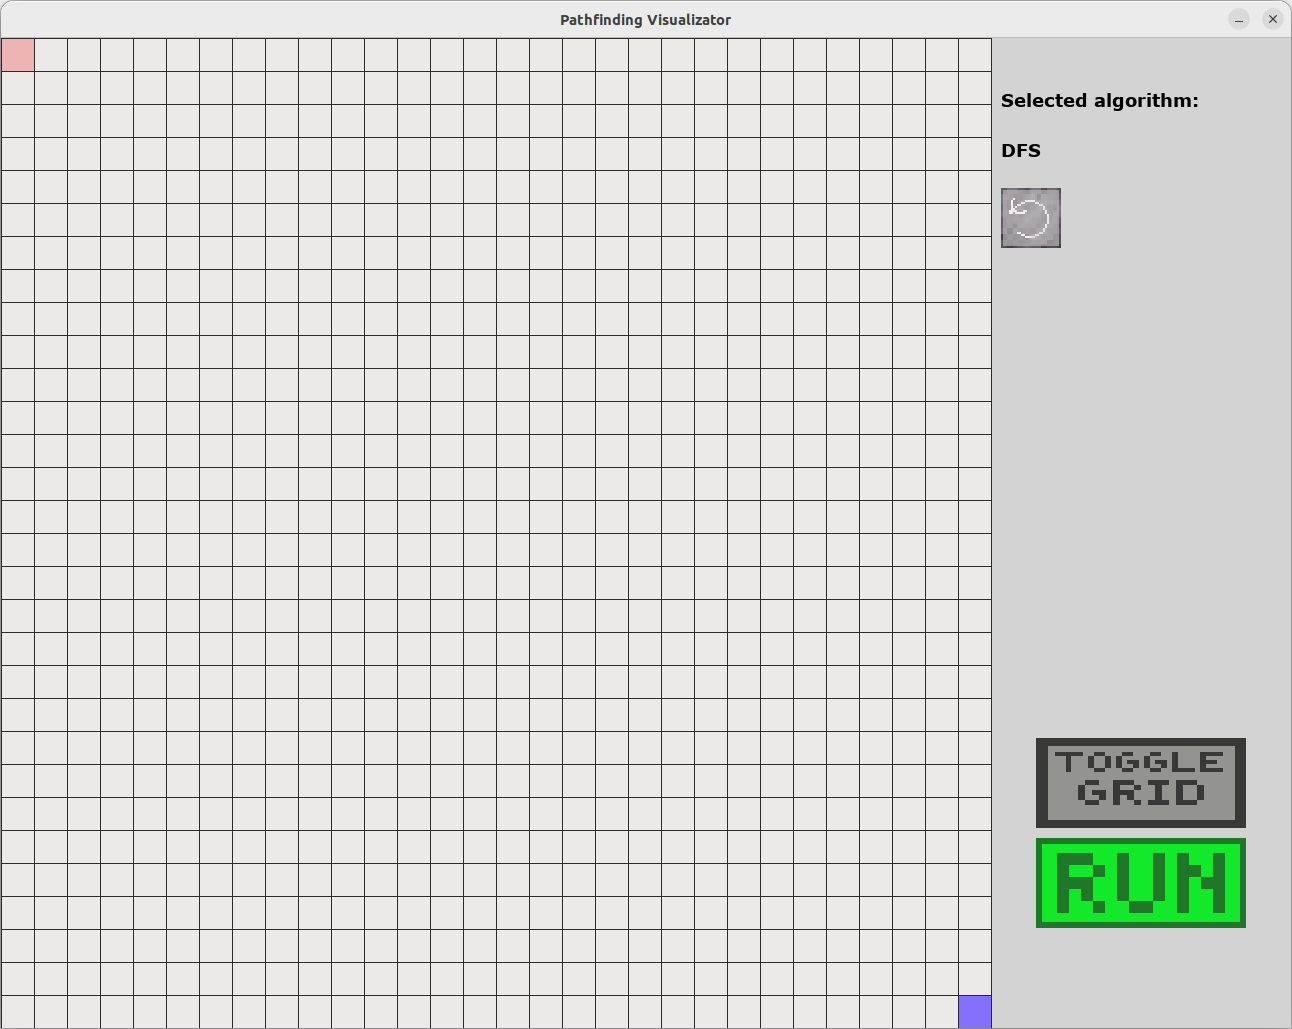
\includegraphics[width = \textwidth]{menu.png}
  			\caption{Hlavní obrazovka}
  			\label{menu}
  			\end{figure}
  			
			\section{Ovládání}
			Nejsnazší a~také nejpohodlnější způsob, jak program ovládat je pomocí klávesnice:
			\begin{itemize}
			
			\setlength\itemsep{0.01mm}
			\item Tlačítky 1, 2, 3, 4 se mění vybraný algoritmus (DFS, BFS, Greedy Best First Search, A*).
\item Mezerník spustí vizualizaci.
\item 'g' vygeneruje bludiště.
\item 's' vybere nástroj pro umisťování startu.
\item 'f' vybere nástroj pro umisťování cíle.
\item 'd' vybere nástroj pro kreslení a~gumování stěn.
\item 'c' smaže políčka vybarvená dokončenou vizualizací.
\item 'i' zapne/vypne barevný mód vizualizace.
\item 'r' restartuje celou aplikaci.
\item Šipka nahoru zpomalí vizualizaci.
\item Šipka dolů zrychlí vizualizaci.

			Kromě tlačítek klávesnice lze některé funkce ovládat i~tlačítky v~postranním panelu aplikace. Konkrétně tlačítko v~horní části vybere další algoritmus v~pořadí, tlačítko \uv{TOGGLE GRID} přepíná vykreslování mřížky a~tlačítko \uv{RUN} spouští vizualizaci. Tyto tlačítka jsem vytvořil, aby bylo možné program na základní úrovni ovládat i~bez znalosti klávesového ovládání.
			
			
			Mimo to lze v~souboru \texttt{settings.py} upravovat pokročilé možnosti. Proměnná \texttt{sideLength} udává počet políček ve straně mřížky. Výchozí hodnotou pro \texttt{sideLength} je 50, program správně vykresluje políčka pro hodnoty \texttt{sideLength} $\leq 990$, což je výchozí počet pixelů ve straně mřížkového prostoru. Pro 990 tak jedno políčko zabírá jeden pixel obrazovky, nastavení vyšší hodnoty má za následek nevykreslení některých políček. Algoritmy stále bude fungovat, jen některé vrcholy grafu se nevykreslí.
			Dále se v~souboru dá nastavit rozlišení okna aplikace a~barvy políček. Je třeba mít na paměti, že nesprávný zásah má za následek dysfunkci programu.
			%Celkový počet políček je tak $\texttt{sideLength}^2$. 
			\end{itemize}
			\section{Barevné označení políček}
			V~programu se při standardní vizualizaci algoritmů používá pro políčka následující barevné označení podle jejich aktuálního stavu: \\[1ex]
			
			\newcommand\ColorSquare[1]{{\color{#1}\rule{4mm}{4mm}}}			
			\definecolor{visited_colour}{RGB}{255,0,0}
			\definecolor{wall_colour}{RGB}{0,0,0}
			\definecolor{start_colour}{RGB}{238,180,180}
			\definecolor{finish_colour}{RGB}{132,112,255}
			\definecolor{path_colour}{RGB}{255,255,0}
			\definecolor{in_frontier_colour}{RGB}{154,205,50}
			\definecolor{empty_colour}{RGB}{238,233,233}	
			
			\begin{minipage}[outer sep=0]{\textwidth}
\begin{minipage}[t]{0.48\textwidth}
značení výchozího stavu:\\
\ColorSquare{start_colour} \quad startovní vrchol \\
			\ColorSquare{finish_colour} \quad cílový vrchol \\
			\ColorSquare{empty_colour} \quad průchozí vrchol\\
			\ColorSquare{wall_colour} \quad neprůchozí vrchol/stěna \\
    \end{minipage}\hfill
    \begin{minipage}[t]{0.48\textwidth}
    značení stavu při vizualizaci:\\
    \ColorSquare{in_frontier_colour} \quad vrchol čekající na expanzi\\ %čekající na prozkoumání svých sousedů.\\
			\ColorSquare{visited_colour} \quad prozkoumaný vrchol\\	
			\ColorSquare{path_colour} \quad vrchol nalezené cesty
    \end{minipage}
    \end{minipage}\vspace{1ex}
						

			
			\section{Ukázky použití}
			Na adrese \url{https://youtu.be/edACN-PVQnI} je dostupné video ukazující několik vizualizací vyprodukovaných vytvořeným programu. Níže jsou ukázané snímky obrazovky dokončených vizualizací každého algoritmu na stejném bludišti. Snímky jsou oříznuté o~boční panel. Další ukázky vizualizace jsou v příloze \ref{priloha_vizualizace}.
			
\begin{figure}
  			\centering
  			\begin{subfigure}[b]{0.48\textwidth}
  			\centering 
  			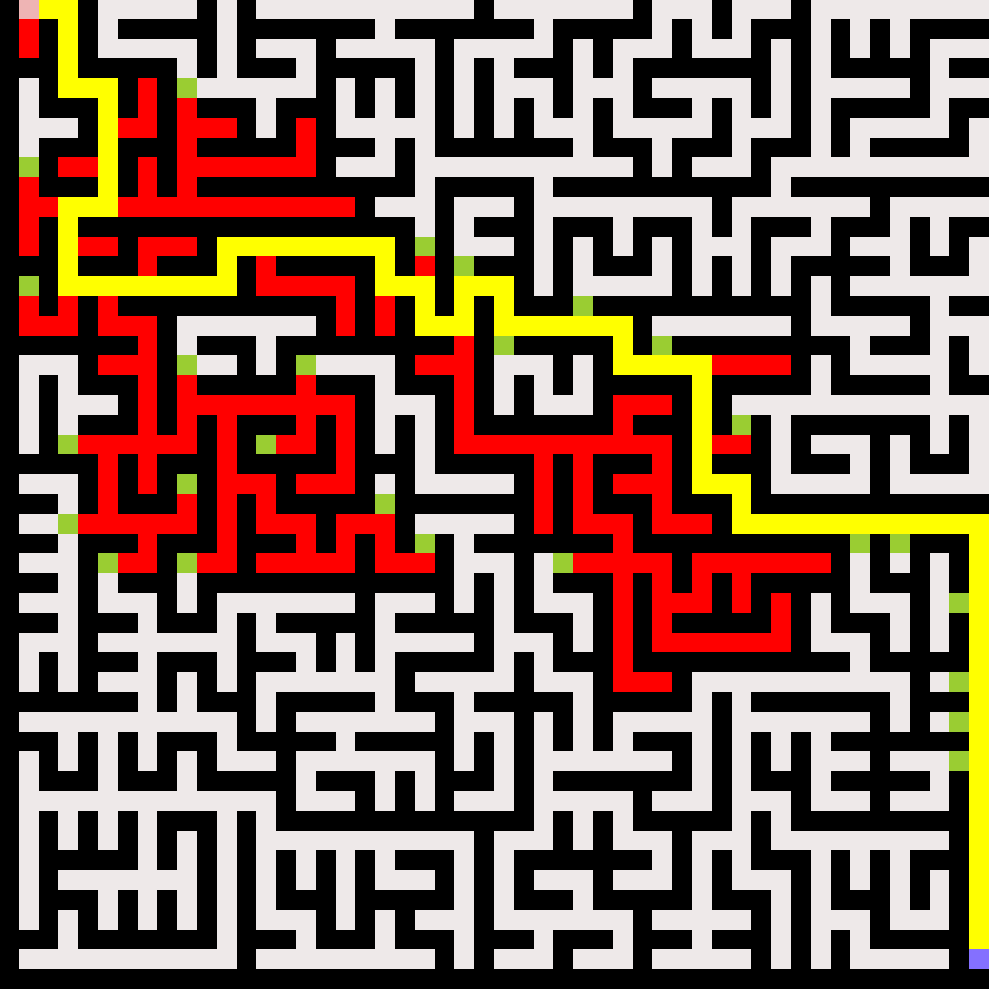
\includegraphics[width=\textwidth]{bludiska/a*1}
  			\caption{}
  			\end{subfigure}
  			\hfill
  			\begin{subfigure}[b]{0.48\textwidth}
    		\centering
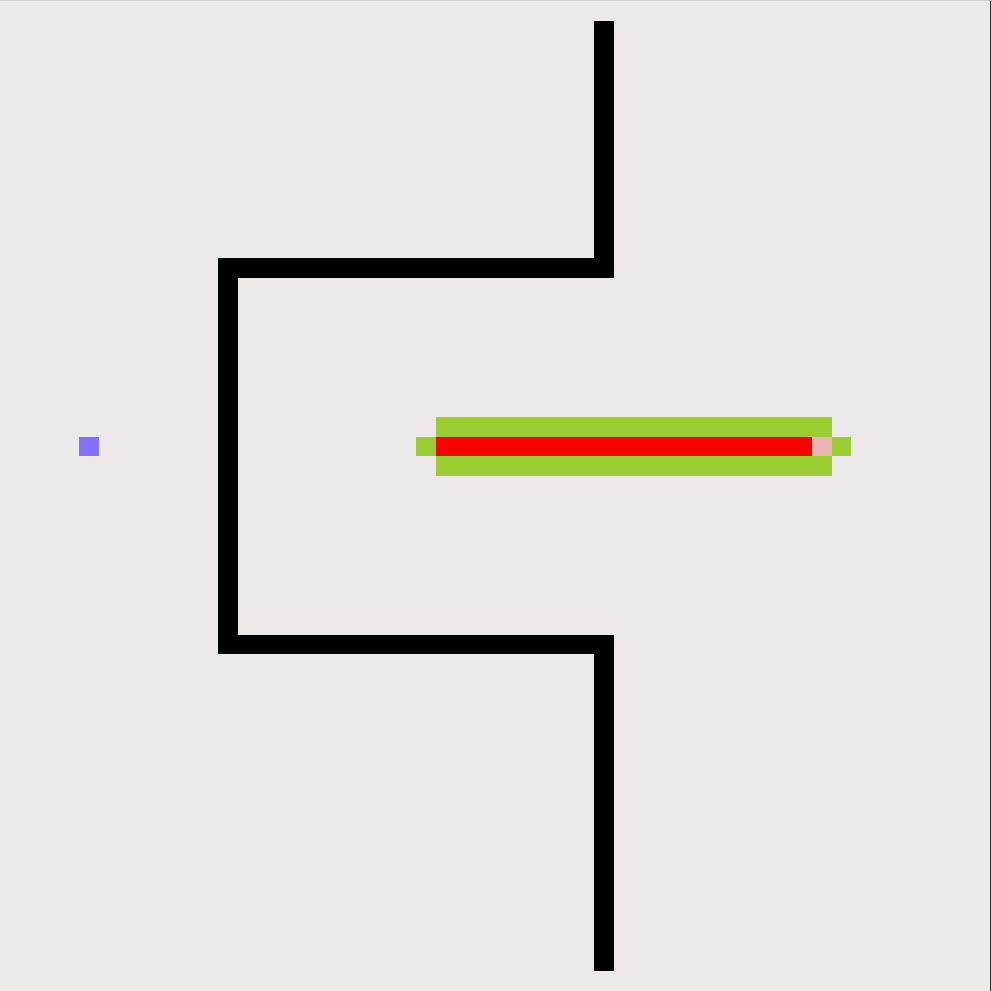
\includegraphics[width=\textwidth]{bludiska/greedy1}
    		\caption{}
  			\end{subfigure}
  			\begin{subfigure}[b]{0.48\textwidth}
    		\centering
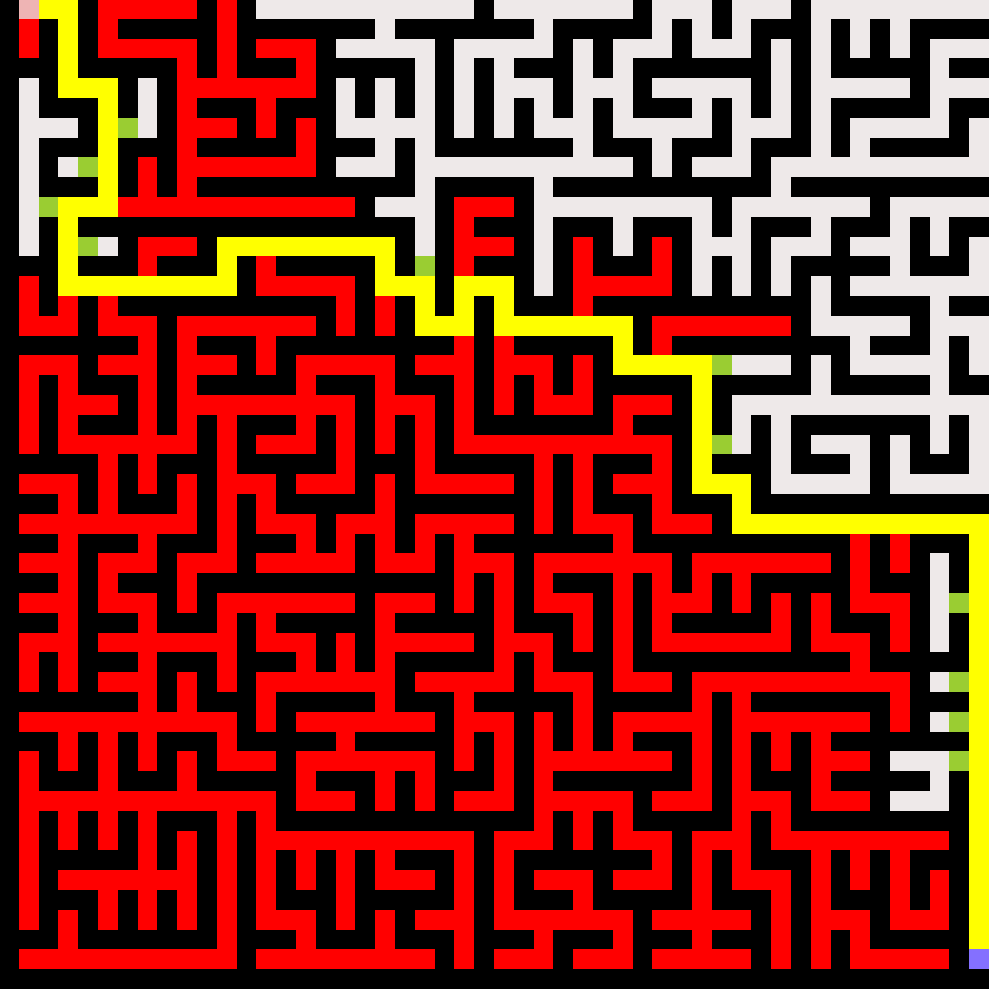
\includegraphics[width=\textwidth]{bludiska/dfs1}\caption{}
\end{subfigure}
\hfill
  			\begin{subfigure}[b]{0.48\textwidth}
    		\centering
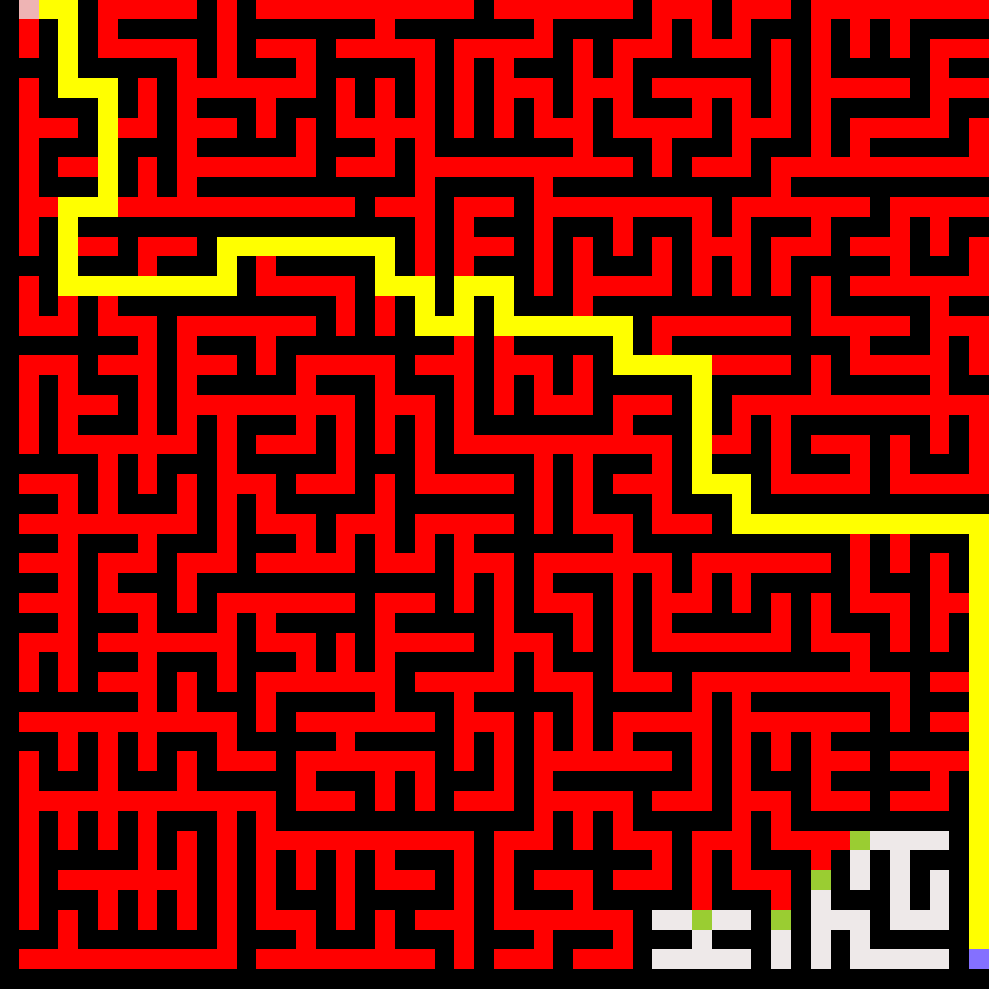
\includegraphics[width=\textwidth]{bludiska/bfs1}
    		\caption{}
  			\end{subfigure}


  \caption{Ukázka vizualizace všech algoritmů na stejném bludišti. (a) A*, (b) hladové vyhledávání, (c) DFS, (d) BFS}
  \label{ukazka_vsechny}
  
\end{figure}			



  			
			


	\chapter*{Závěr}
	
	V teoretické části jsem čtenáře nejprve seznámil s pojmem algoritmus jako takovým, dále jsem se zaměřil na teoretické principy týkající se algoritmů obecně.  
	
	Hlavním přínosem teoretické části je pak obsáhlý přehled významných algoritmů pro vyhledávání cest. V práci byly shrnuty jejich charakteristické vlastnosti a bylo objasněno jakým způsobem fungují. Navíc byla část doplněna i některými poznatky z teorie grafů umožňující ucelený pohled na celou problematiku.
	
	%Dále jsem se zaměřil na komplexní různých algoritmů na vyhledání cest
		%V~teoretické části práce jsem čtenáře seznámil s~pojmy týkajících se algoritmů, dále byly shrnuty základy 
		%jsem představil některé významné algoritmy z~oblasti pathfinding. 
		V~hlavní části práce se mi podařilo implementovat vizualizační program, který názorně vizualizuje chod algoritmů z~první části. Program umožňuje uživateli nastavit si důležité parametry, jako je jaký algoritmus má být vizualizován, rychlost vizualizace nebo vstup pro algoritmus. Program má jednoduché ovládání a~vykresluje všechny důležité informace na obrazovku. Navíc je doplněn i~o~několik užitečných prvků, jako je generování náhodného bludiště nebo přepínání zobrazení mřížky.
		
		Nejzávažnějším problémem programu je, že při nastavení velké mřížky mají některé funkce programu poměrně velkou odezvu, načtení programu trvá kolem 2 sekund a~přebarvení všech políček vybarvených dokončenou vizualizací podobně. Důvodem je, že kód není vhodně optimalizovaný na takovéto rozměry mřížky. Přesto je i~na nich použitelný.
		
		Program by mohl sloužit jako učební pomůcka například při výkladu algoritmů na hodinách informatiky.
		
		Do budoucna by bylo možné rozšířit program o menu Nápověda, které by vysvětlovalo vizualizované algoritmy a~ovládání programu, nebo o funkcionalitu pro ukládání a~nahrávání vlastních bludišť.
	
	%přidat do vizualizace zvuk, 
	
	\nocite{*}
    \printbibliography					% Vytvoří seznam literatury
	\addcontentsline{toc}{chapter}{Bibliografie}
    \printglossary[title={Zkratky}]		% Vytvoří seznam zkratek
    \listoffigures						% Vytvoří seznam obrázků
    \listoftables						% Vytvoří seznam tabulek
	\listofalgorithms
    \begin{appendices}
    \chapter*{Seznam souborů v~přiloženém ZIP archivu}
    \begin{enumerate}
    \item \texttt{main.py}
    \item \texttt{settings.py}
    \item \texttt{sidebar.py}
	\item \texttt{tile.py}
    \item \texttt{tools.py}
	\item \texttt{vizualizator.py}
	\item složka  \texttt{images}: Obsahuje obrázky tlačítek.
    \end{enumerate}
	\chapter{Ukázky vizualizací}\label{priloha_vizualizace}
	
\begin{figure}[h]
\begin{minipage}[outer sep=0]{\textwidth}
\begin{minipage}[t]{0.45\textwidth}
			
			
\includegraphics[width=\textwidth]{dfs_user}\caption{Vizualizace DFS v~nakresleném grafu. Ukazuje neoptimalitu DFS.}\label{dfs_user}
			
    \end{minipage}\hfill
    \begin{minipage}[t]{0.45\textwidth}

\includegraphics[width=\textwidth]{bfs2_user}\caption{Vizualizace BFS na nakresleném grafu.}\label{bfs2_user}
    \end{minipage}
    \end{minipage}\vspace{1ex}
    
    \begin{minipage}[outer sep=0]{\textwidth}
\begin{minipage}[t]{0.45\textwidth}
			
			
\includegraphics[width=\textwidth]{cropped2/dfsNOWALL}\caption{Vizualizace DFS v bludišti bez překážek.}\label{dfs_user}
			
    \end{minipage}\hfill
    \begin{minipage}[t]{0.45\textwidth}
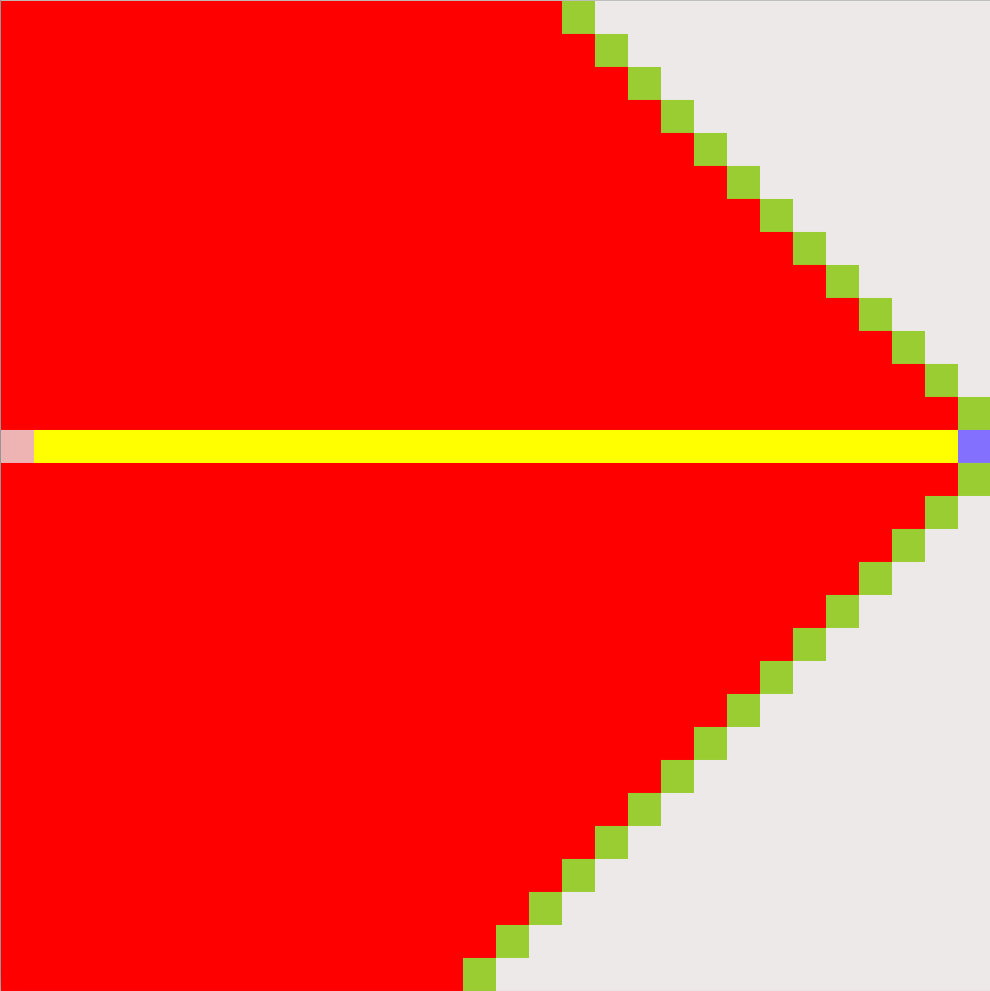
\includegraphics[width=\textwidth]{cropped2/bfsNOWALL}\caption{Vizualizace BFS v bludišti bez překážek.}\label{bfs2_user}
    \end{minipage}
    \end{minipage}\vspace{1ex}
    
    
\end{figure}	








\begin{figure}[h]
\begin{minipage}[outer sep=0]{\textwidth}
\begin{minipage}[t]{0.45\textwidth}
			
			
\includegraphics[width=\textwidth]{cropped2/A*NOWALL}\caption{Vizualizace A* v bludišti bez překážek.}
			
    \end{minipage}\hfill
    \begin{minipage}[t]{0.45\textwidth}

\includegraphics[width=\textwidth]{cropped2/A*NOWALL}\caption{Vizualizace hladového uspořádaného vyhledávání v bludišti bez překážek.}
    \end{minipage}
    \end{minipage}\vspace{1ex}
    
    \begin{minipage}[outer sep=0]{\textwidth}
\begin{minipage}[t]{0.45\textwidth}
			
			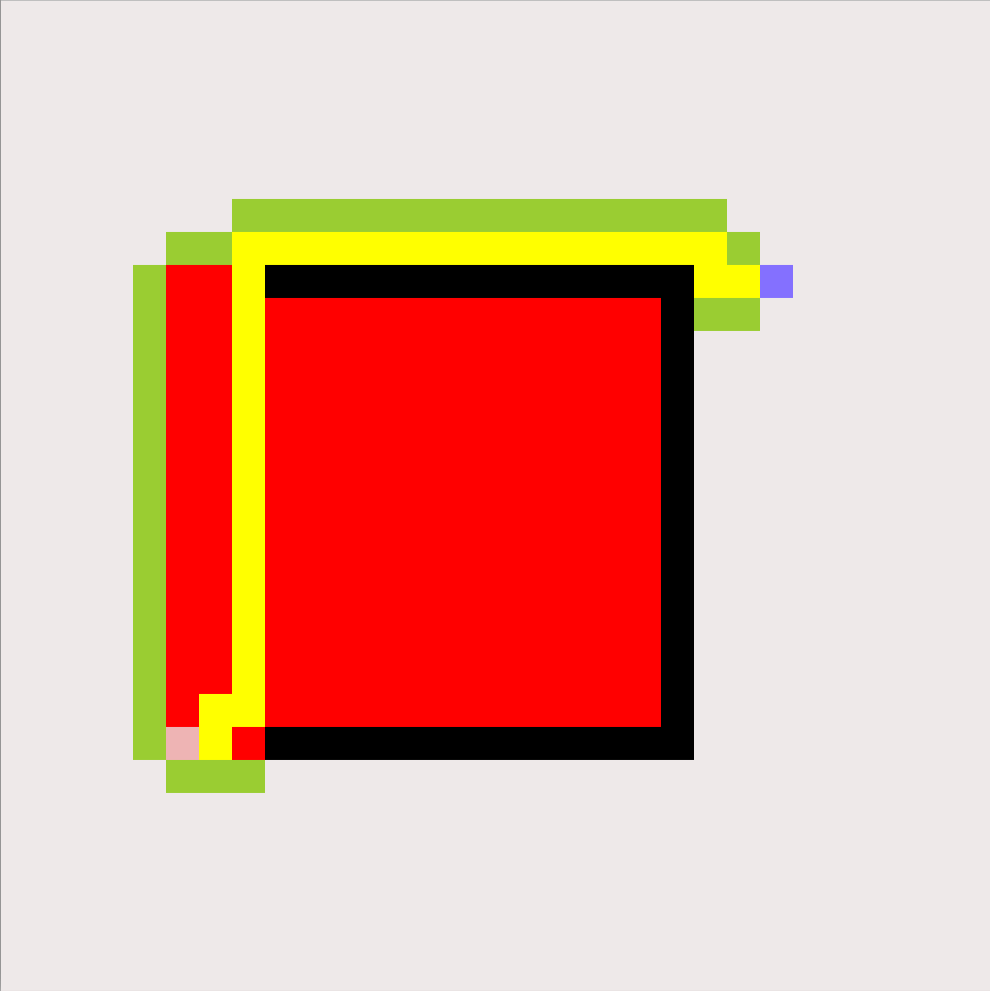
\includegraphics[width=\textwidth]{cropped3/A*WALL}\caption{Vizualizace A* v bludišti s jednoduchou překážkou. }\label{dfs_user}
			
    \end{minipage}\hfill
    \begin{minipage}[t]{0.45\textwidth}

\includegraphics[width=\textwidth]{cropped3/GBFSWALL}\caption{Vizualizace hladového vyhledávání v bludišti s jednoduchou překážkou. Prozkoumá méně polí než A*, ale negarantuje optimální cestu.}\label{bfs2_user}
    \end{minipage}
    \end{minipage}\vspace{1ex}
    
    
\end{figure}	










\begin{figure}
  			\centering 
  			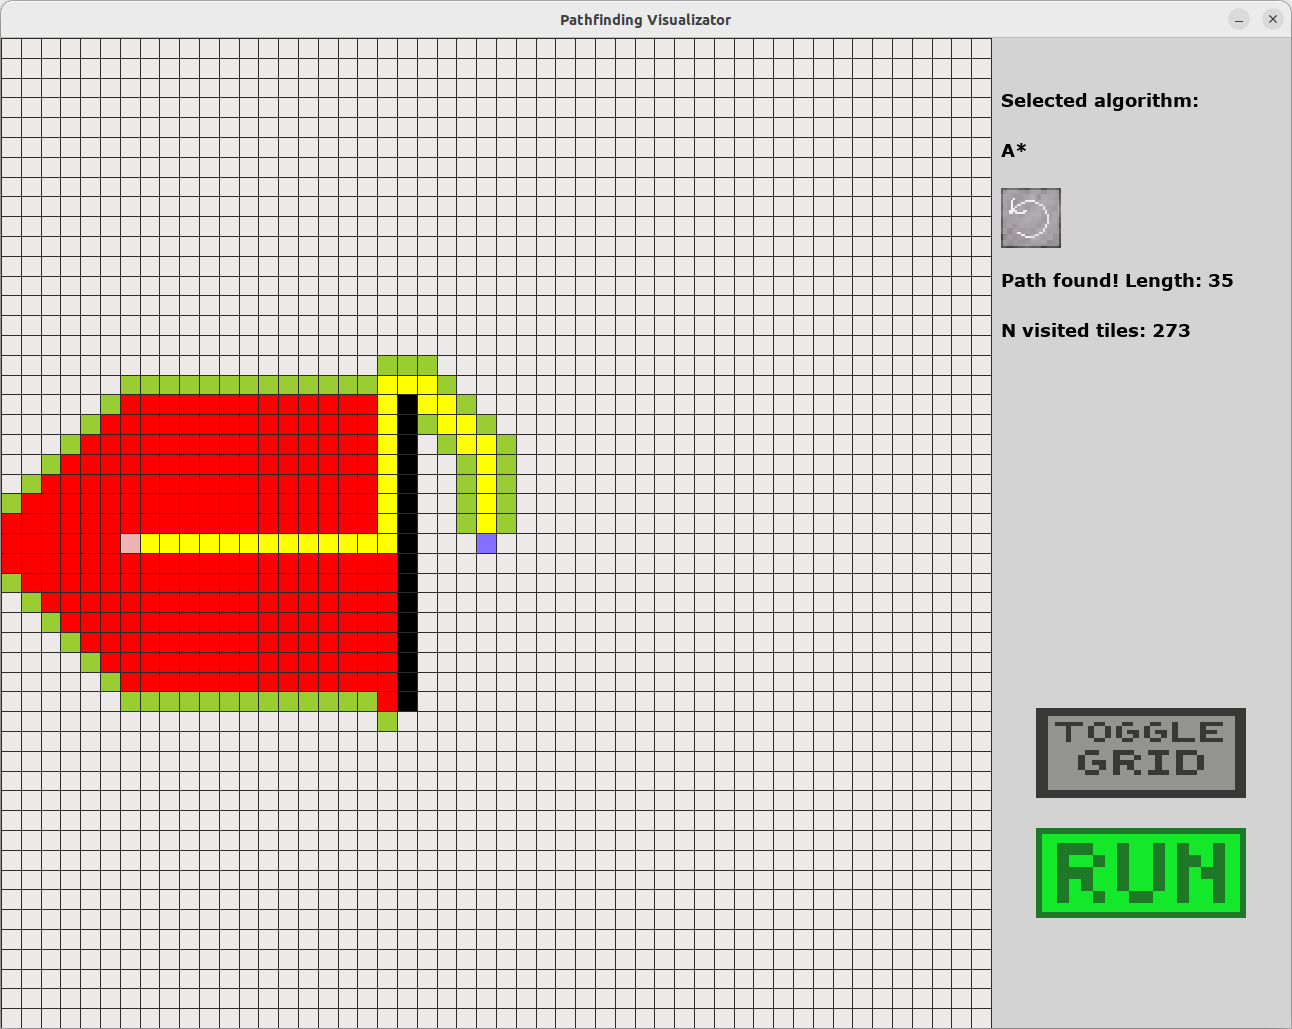
\includegraphics[width = 14cm]{vizu_hotova.png}
  			\caption{Celé okno s~doběhlou vizualizací A*}
  			\label{vizu1}
  			\end{figure}
  			
  			
\begin{figure}[h]
\begin{minipage}[outer sep=0]{\textwidth}
\begin{minipage}[t]{0.48\textwidth}
			
  			
\includegraphics[width=\textwidth]{Iuser_gbfs}\caption{Vizualizace hladového uspořádaného vyhledávání v~nepříznivém grafu. Algoritmus se nechá \uv{zlákát} do lokálního minima a~nenajde nejkratší cestu.}\label{gbfs_user}
			
    \end{minipage}\hfill
    \begin{minipage}[t]{0.48\textwidth}
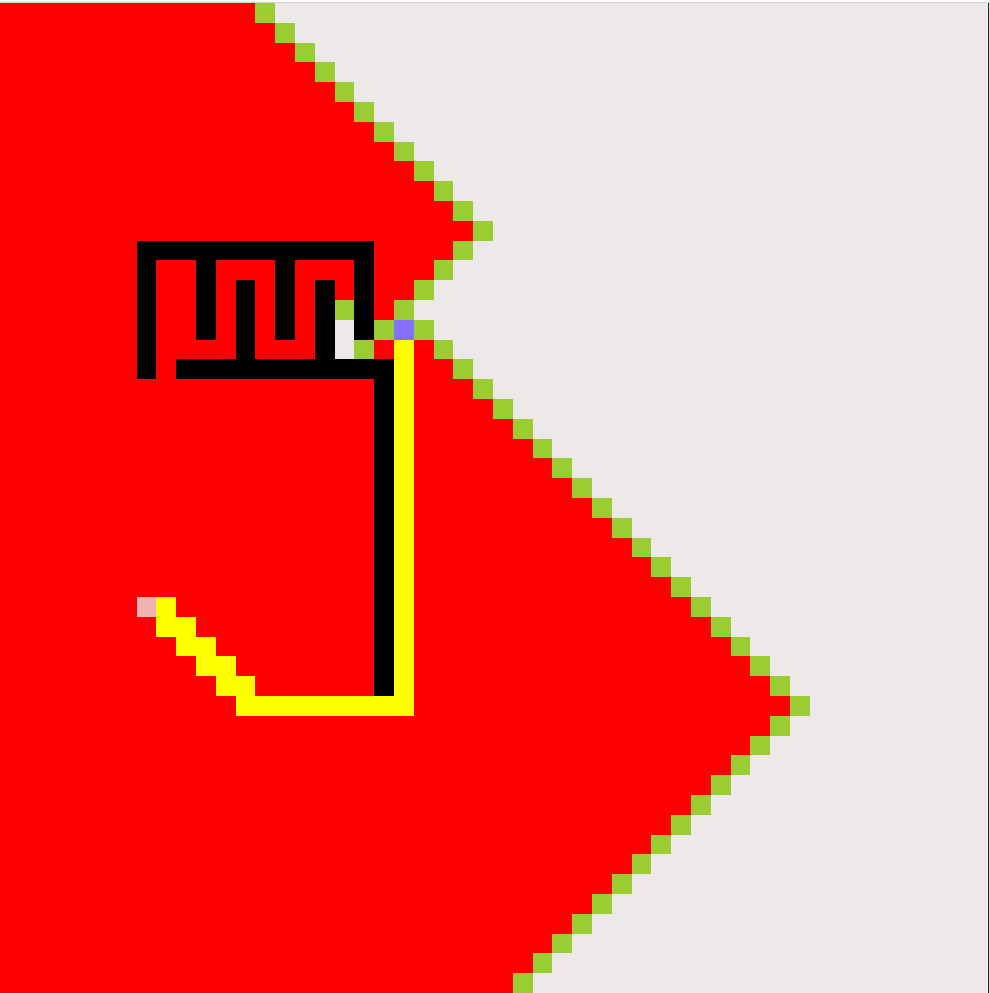
\includegraphics[width=\textwidth]{Ibfs_user}\caption{Dokončená vizualizace BFS na grafu z obr. \ref{gbfs_user}. BFS prohledá více polí, ale garantuje nejkratší cestu.}\label{bfs_user}
    \end{minipage}
    \end{minipage}\vspace{1ex}
\end{figure}






	
%\begin{figure}[h]
  			%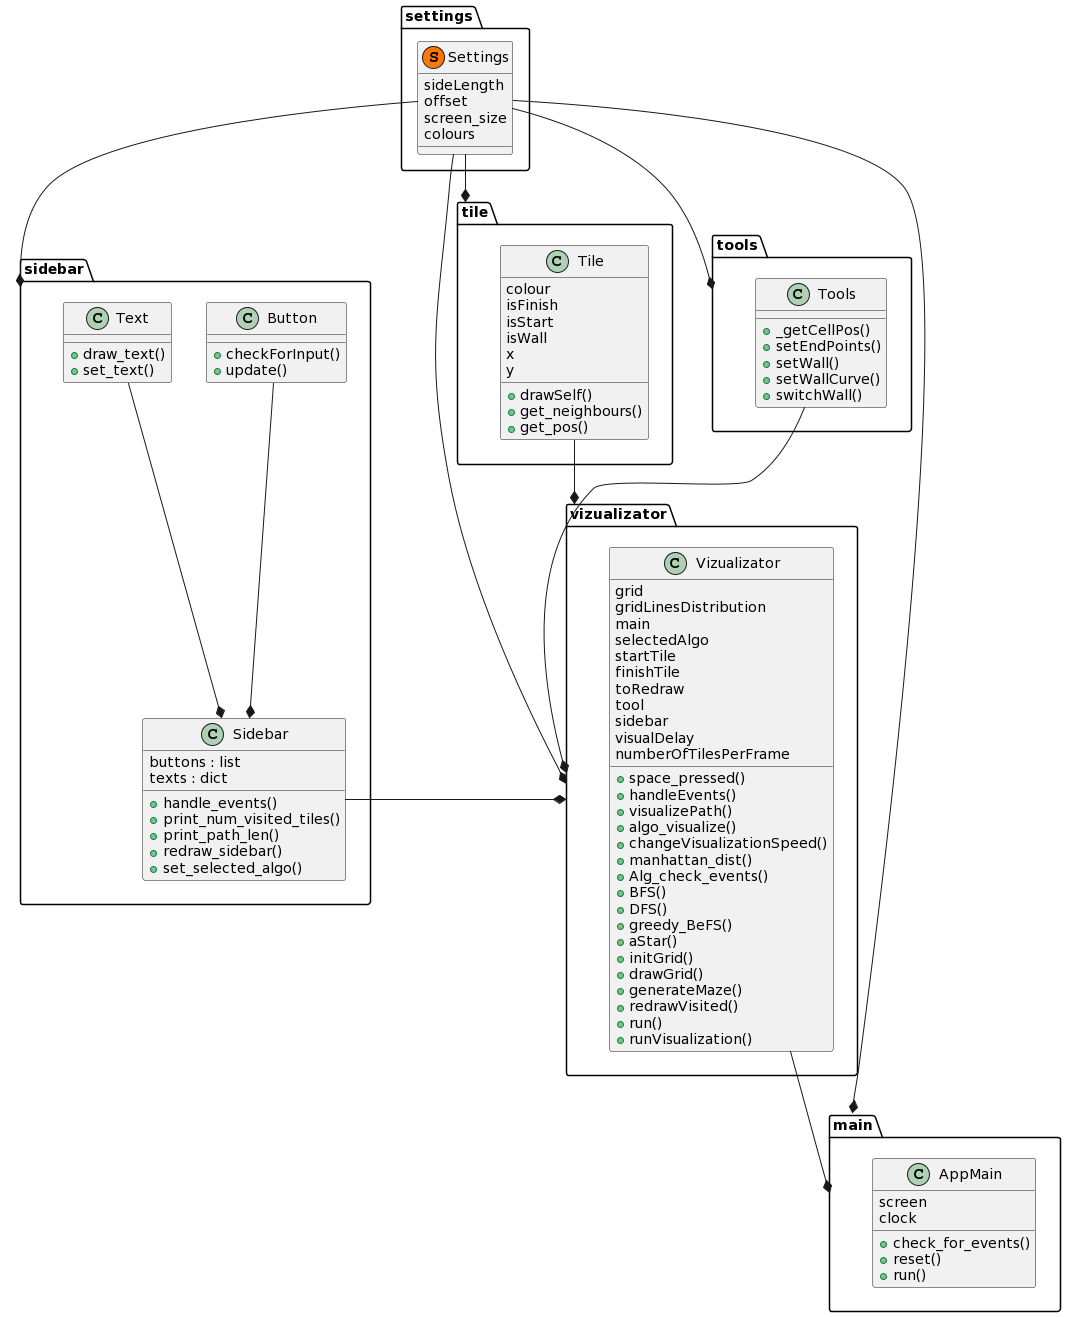
\includegraphics[height=\textwidth,angle=90,origin=c]{diagram1}\caption{Diagram modulů a~tříd}\label{app_diagram}\end{figure}
	\chapter{Implementované algoritmy}\label{idk}
	
	\begin{lstlisting}[caption={Algoritmus DFS},captionpos=b]
	def DFS(self):
        """Depth First Search"""
        visited = set()
        stack = [self.startTile]
        parentDict = dict()
        parentDict[self.startTile] = None
        visited.add(self.startTile)
        i = 0 # Iteration counter
        while stack:
            self.Alg_check_events()
            current = stack.pop()

            if current == self.goalTile:
                return parentDict, True

            self.setCurrsColour(current, parentDict)

            # Add neighbors to the stack
            for neighbor in current.get_neighbours(self.grid):
                if neighbor not in visited:
                    if neighbor != self.startTile and neighbor != self.goalTile:
                        neighbor.colour = settings.in_frontier_colour
                        neighbor.drawSelf(self.main.screen)

                    stack.append(neighbor)
                    parentDict[neighbor] = current
                    visited.add(neighbor)

            # Update the screen with newly drawn tiles based on visualization speed
            i = self.algo_visualize(i)

        # If stack got emptied but goal was not found there is no path 
        return parentDict, False
	\end{lstlisting}
	\newpage
					\begin{lstlisting}[caption={Algoritmus BFS},captionpos=b]
    def BFS(self):
        """Breadth First Search"""
        visited = set()
        queue = deque()
        queue.appendleft(self.startTile)
        parentDict = dict()
        parentDict[self.startTile] = None
        visited.add(self.startTile)
        i = 0 # Iteration counter
        while queue:
            self.Alg_check_events()
            current = queue.pop()
            
            if current == self.goalTile:
                return parentDict, True

            self.setCurrsColour(current, parentDict)

            # Enqueue neighbors
            for neighbor in current.get_neighbours(self.grid):
                if neighbor not in visited:
                    if neighbor != self.startTile and neighbor != self.goalTile:
                        neighbor.colour = settings.in_frontier_colour
                        neighbor.drawSelf(self.main.screen)
                        
                    queue.appendleft(neighbor)
                    parentDict[neighbor] = current
                    visited.add(neighbor)
                    
            # Update the screen with newly drawn tiles based on visualization speed
            i = self.algo_visualize(i)

        # If queue got emptied but goal was not found there is no path 
        return parentDict, False
		\end{lstlisting}
		\newpage
		\begin{lstlisting}[caption={Algoritmus greedy best-first search},captionpos=b]
		def greedy_BeFS(self):
        """Greedy Best First Search"""

        # Define priority queue item as (heuristic, node) tuple
        @dataclass(order=True)
        class PrioritizedItem: 
            priority: int
            item: Any = field(compare=False)

        visited = set()
        priority_queue = PriorityQueue() 
        priority_queue.put(PrioritizedItem(priority=0, item=self.startTile)) 

        parentDict = dict()
        parentDict[self.startTile] = None
        visited.add(self.startTile)
        i = 0 # Iteration counter
        while not priority_queue.empty():
            self.Alg_check_events()
            current = priority_queue.get().item

            if current == self.goalTile:
                return parentDict, True

            self.setCurrsColour(current, parentDict)

            # Add neighbors to priority queue
            for neighbor in current.get_neighbours(self.grid):
                if neighbor not in visited:
                    if neighbor != self.startTile and neighbor != self.goalTile:
                        neighbor.colour = settings.in_frontier_colour
                        neighbor.drawSelf(self.main.screen)

                    priority = self.manhattan_dist(neighbor, self.goalTile)
                    priority_queue.put(PrioritizedItem(priority=priority, item=neighbor))
                    parentDict[neighbor] = current
                    visited.add(neighbor)

            # Update the screen with newly drawn tiles based on visualization speed
            i = self.algo_visualize(i)

        # If priority queue got emptied but goal was not found there is no path
        return parentDict, False
		\end{lstlisting}
		\newpage
		\begin{lstlisting}[language = Python, caption={Algoritmus A*},captionpos=b]
		def aStar(self):
        """A* algorithm"""

        # Define priority queue item as (heuristic, h_score, node) tuple
        @dataclass(order=True)
        class PrioritizedItem:
            priority: int
            h_score: int # Often there are many nodes with the same priority in Priority Q.;breaking ties on lower h results in A* expanding to get closer to the goal ASAP while maintaining optimality  
            item: Any = field(compare=False)

        visited = set()
        priority_queue = PriorityQueue()
        f_score_start = self.manhattan_dist(self.startTile, self.goalTile)
        priority_queue.put(PrioritizedItem(priority=0, h_score=f_score_start, item=self.startTile))
        parentDict = dict()
        parentDict[self.startTile] = None
        visited.add(self.startTile)
        closed = set()
        g_cost_dict = dict()
        g_cost_dict[self.startTile] = 0
        i = 0 # Iteration counter
        while not priority_queue.empty():
            self.Alg_check_events()
            current = priority_queue.get().item
            if current not in closed: 

                if current == self.goalTile:
                    return parentDict, True
                
                self.setCurrsColour(current, parentDict)

                #Add neighbors to priority queue
                for neighbor in current.get_neighbours(self.grid):
                    g_cost = g_cost_dict[current] + 1 # Setting g_cost to be always 0 would turn A* into Greedy best first search
                    h_cost = self.manhattan_dist(neighbor, self.goalTile) # Setting h_cost to be always 0 would turn A* into Uniform Cost Search
                    f_cost = g_cost + h_cost

                    if neighbor not in visited:
                        if neighbor != self.startTile and neighbor != self.goalTile:
                            neighbor.colour = settings.in_frontier_colour
                            neighbor.drawSelf(self.main.screen)
                            
                        priority_queue.put(PrioritizedItem(priority=f_cost, h_score=h_cost, item=neighbor))
                        g_cost_dict[neighbor] = g_cost
                        parentDict[neighbor] = current
                        visited.add(neighbor)

                    elif g_cost < g_cost_dict[neighbor]:
                        # This path is better than the old one (better g cost), update the priority queue; leaves old item with worse priorty in PQ, that gets resolved by closed list
                        priority_queue.put(PrioritizedItem(priority=f_cost, h_score=h_cost, item=neighbor)) 
                        g_cost_dict[neighbor] = g_cost
                        parentDict[neighbor] = current
                
                #Update the screen with newly drawn tiles based on visualization speed
                i = self.algo_visualize(i)
                closed.add(current)

        # If priority queue got emptied but goal was not found there is no path
        return parentDict, False
		\end{lstlisting}
	\end{appendices}
\end{document}
